%!TEX root = ./template-skripsi.tex
%-------------------------------------------------------------------------------
%                            BAB IV
%               		HASIL DAN PEMBAHASAN
%-------------------------------------------------------------------------------

\chapter{HASIL DAN PEMBAHASAN}
    \section{Input Video}
        Pada tahap pertama, sumber data berupa video dimasukkan kedalam sistem yang kemudian diubah menjadi sekumpulan citra \textit{(frame)}. Kemudian citra melalui proses \textit{pre-processing}, yaitu konversi ruang warna RGB ke ruang warna \textit{grayscale}.
        \vspace{-0.5cm}
        \begin{figure}[H]
        \centering
          \singlespacing
          \captionsetup{justification=centering,margin=0.5cm}
          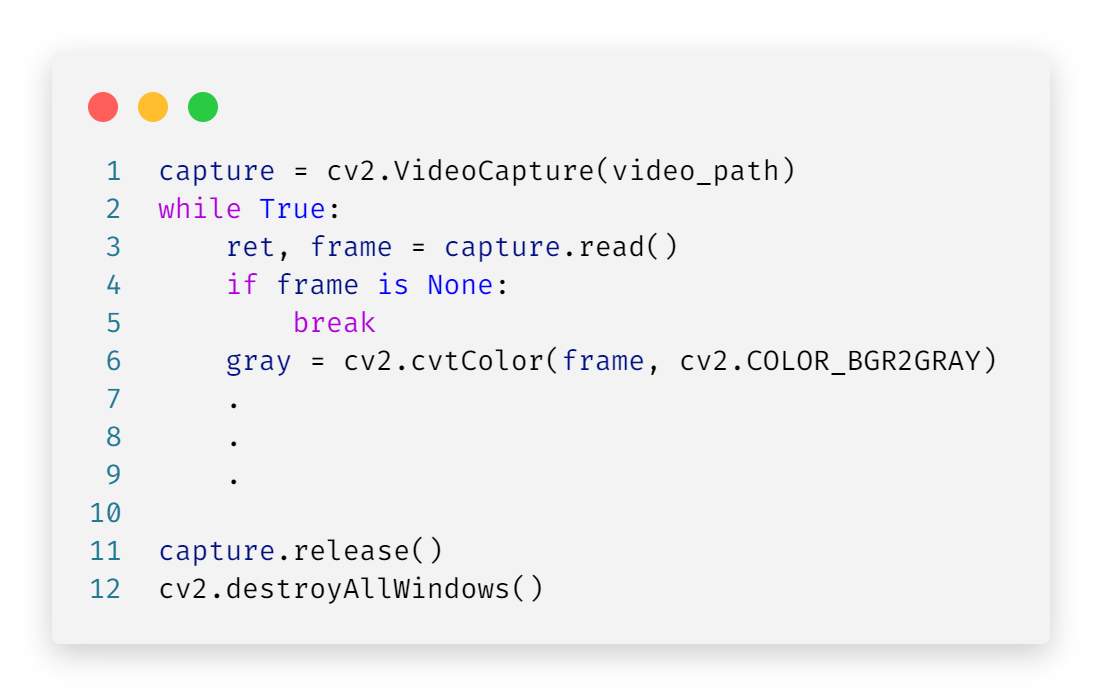
\includegraphics[width=12cm]{image/input.png}
          \caption{Potongan sampel kode input sistem}
          \label{fig:Potongan sampel kode input sistem}
        \end{figure}

    \section{GMM}
        Citra yang telah melalui proses \textit{pre-processing} selanjutnya digunakan sebagai data masukan proses \textit{background subtraction} menggunakan GMM. Keluaran dari metode ini kemudian dievaluasi terhadap \textit{groundtruth} yang sudah dipersiapkan sebelumnya. Diperoleh skor \textit{accuracy, recall, precision,} dan \textit{F1} untuk masing-masing data uji.

        \vspace{-0.5cm}
        \begin{figure}[H]
        \centering
          \singlespacing
          \captionsetup{justification=centering,margin=0.5cm}
          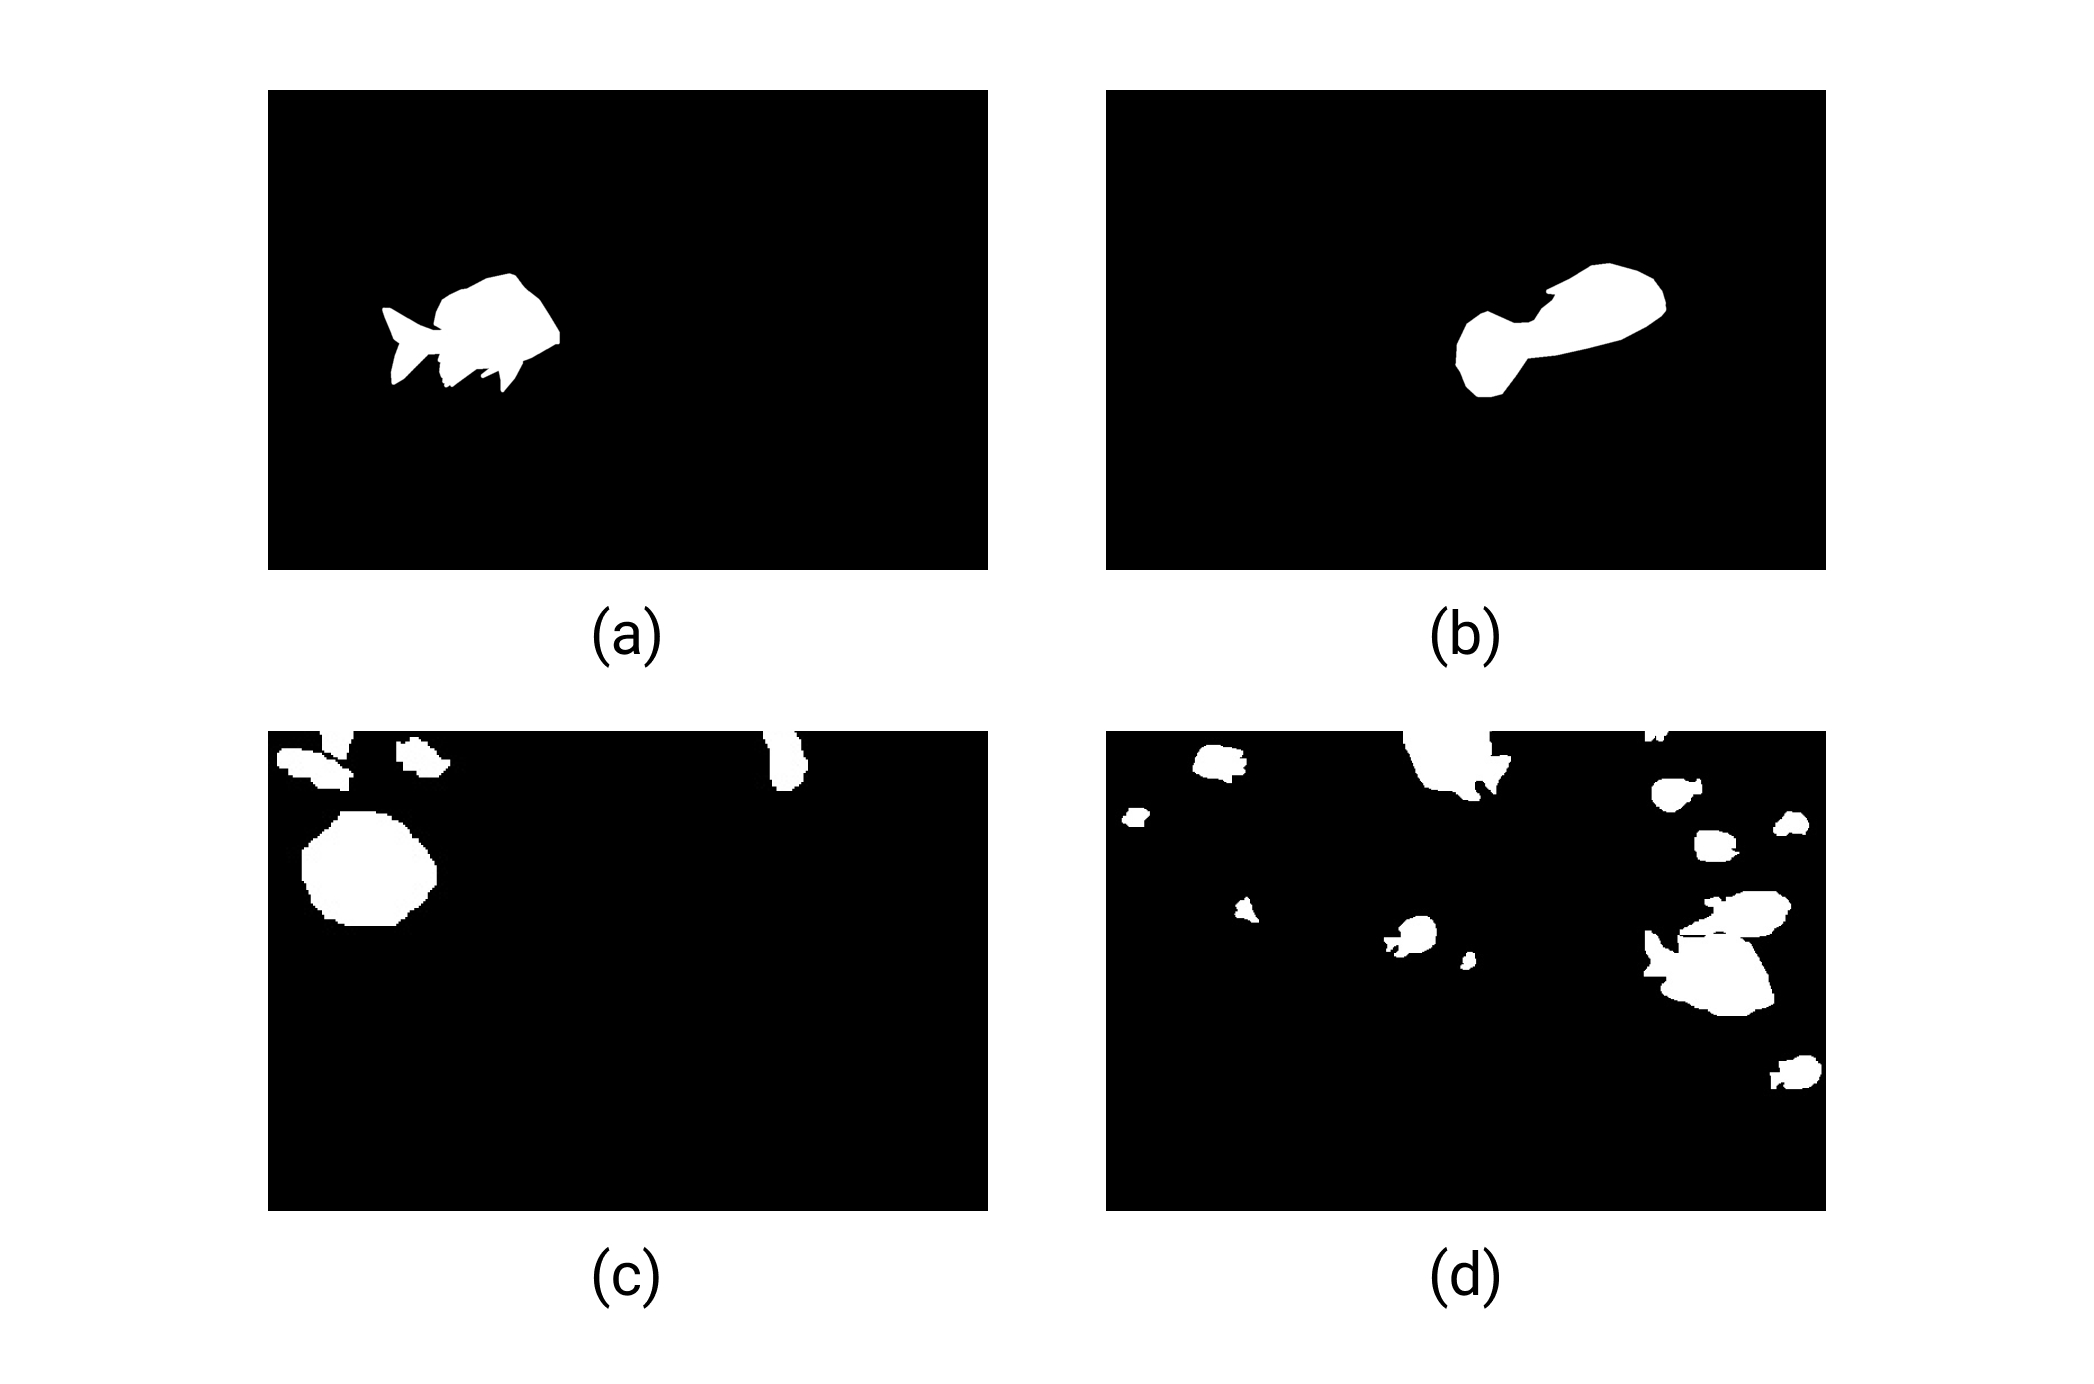
\includegraphics[width=14cm]{image/sample_groundtruth.jpg}
          \caption{Sampel \textit{groundtruth} data uji video indeks (a) 9908 (b) 9866 (c) gt\textunderscore124 (d) gt\textunderscore116}
          \label{fig:sample_groundtruth}
        \end{figure}

        Tabel \ref{tab:gmm_9908} memperlihatkan hasil dari dataset video kategori objek tunggal latar belakang sederhana. Untuk kategori video tersebut, dataset yang digunakan dapat dikatakan kurang optimal. Skor performa cenderung fluktuatif dikarenakan terlalu banyak \textit{noise} yang dihasilkan, serta jumlah frame yang sedikit.

        \begin{longtblr}[
            caption = {Hasil ujicoba proses \textit{background subtraction} menggunakan GMM terhadap video indeks 9908},
            label = {tab:gmm_9908}
        ]{
            colspec={|c|c|c|c|c|},
            rowhead=1
        }
            \hline
            Frame & Citra Asli & Hasil GMM & Groundtruth & \textit{F1} \\ \hline
            120 &
            \begin{minipage}{0.24\textwidth}
                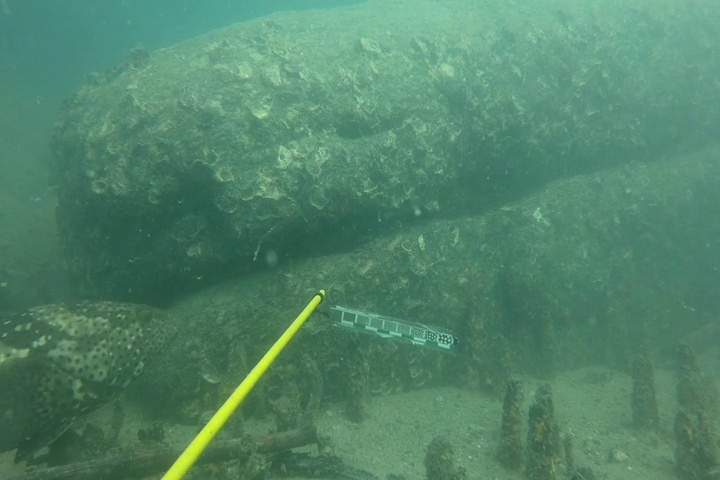
\includegraphics[width=\linewidth]{image/9908/9908_original_frame120.jpg}
            \end{minipage} &
            \begin{minipage}{0.24\textwidth}
                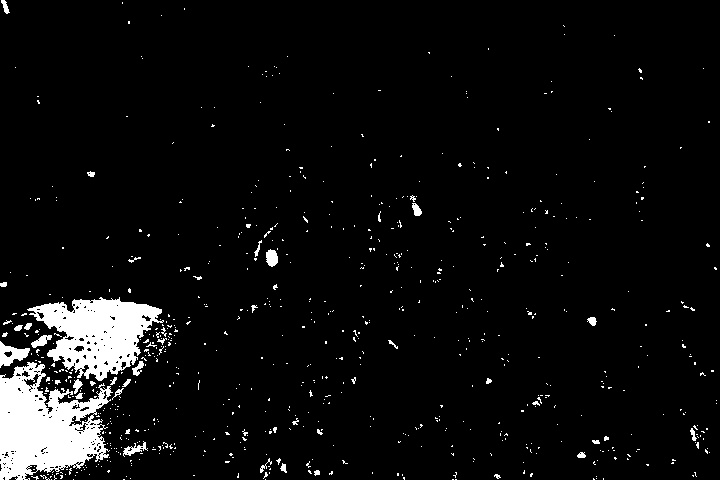
\includegraphics[width=\linewidth]{image/9908/9908_gmm_frame120.jpg}
            \end{minipage} &
           \begin{minipage}{0.24\textwidth}
           	
\includegraphics[width=\linewidth]{image/9908/9908_groundtruth_120.png}
           \end{minipage} &
            58 \\ \hline
            230 &
            \begin{minipage}{0.24\textwidth}
                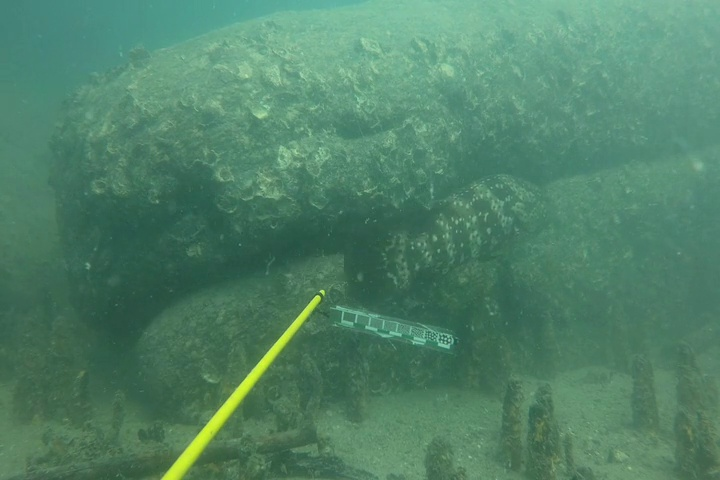
\includegraphics[width=\linewidth]{image/9908/9908_original_frame230.jpg}
            \end{minipage} &
            \begin{minipage}{0.24\textwidth}
                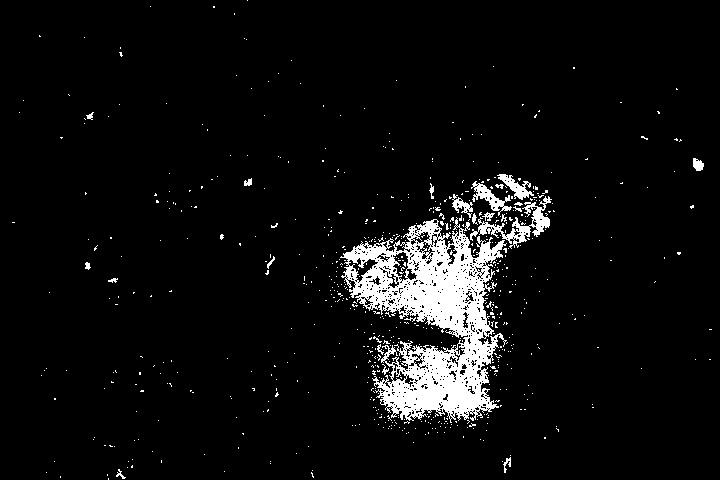
\includegraphics[width=\linewidth]{image/9908/9908_gmm_frame230.jpg}
            \end{minipage} &
            \begin{minipage}{0.24\textwidth}
            	
\includegraphics[width=\linewidth]{image/9908/9908_groundtruth_230.png}
            \end{minipage} &
            31,8 \\ \hline
            290 &
            \begin{minipage}{0.24\textwidth}
                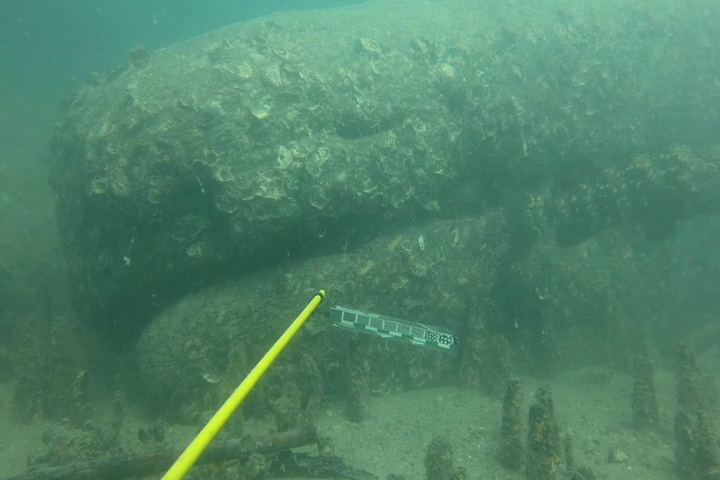
\includegraphics[width=\linewidth]{image/9908/9908_original_frame290.jpg}
            \end{minipage} &
            \begin{minipage}{0.24\textwidth}
                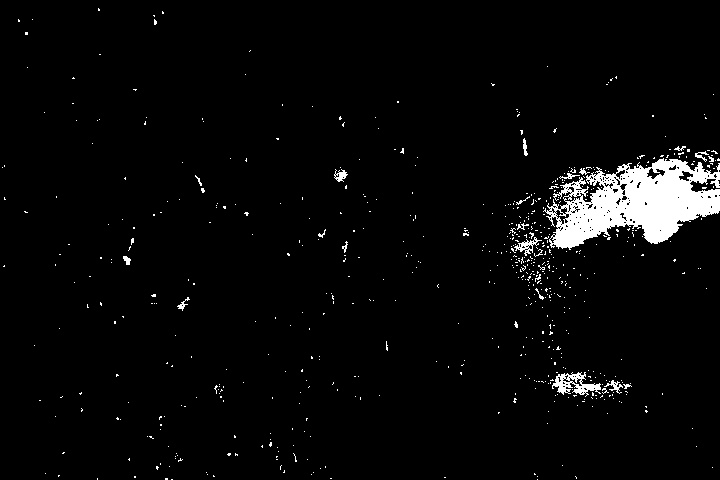
\includegraphics[width=\linewidth]{image/9908/9908_gmm_frame290.jpg}
            \end{minipage} &
            \begin{minipage}{0.24\textwidth}
            	
\includegraphics[width=\linewidth]{image/9908/9908_groundtruth_290.png}
            \end{minipage} &
            58,4 \\ \hline
        \end{longtblr}
    
    	\vspace{1.5cm}

        \begin{longtblr}[
            caption = {Hasil ujicoba proses \textit{background subtraction} menggunakan GMM terhadap video indeks 9986},
            label = {tab:gmm_9986}
        ]{
            colspec={|c|c|c|c|c|c|c|},
            rowhead=1
        }
            \hline
            Frame & Citra Asli & Hasil GMM & Groundtruth & \textit{F1} \\ \hline
            509 &
            \begin{minipage}{0.24\textwidth}
                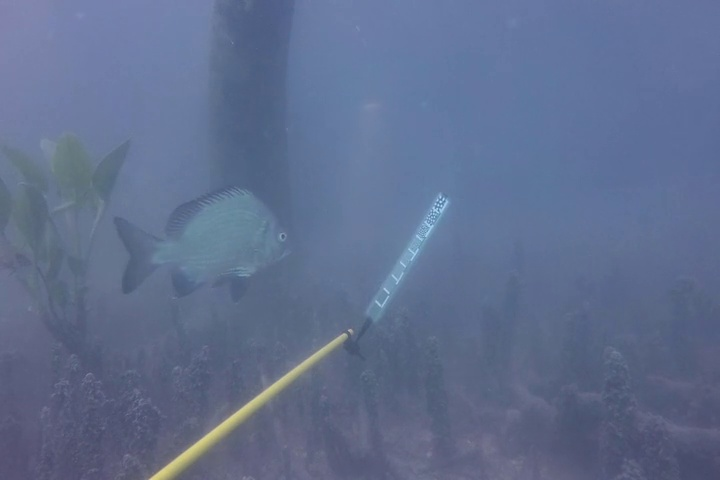
\includegraphics[width=\linewidth]{image/9866/9866_original_frame509.jpg}
            \end{minipage} &
            \begin{minipage}{0.24\textwidth}
                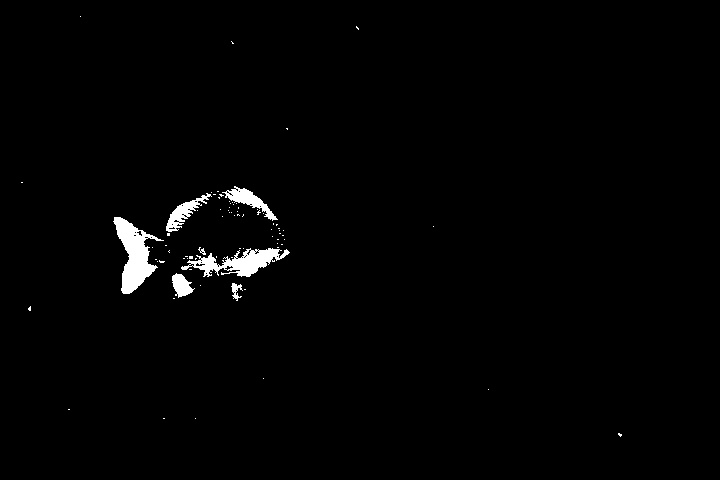
\includegraphics[width=\linewidth]{image/9866/9866_gmm_frame509.jpg}
            \end{minipage} &
           \begin{minipage}{0.24\textwidth}
           	
\includegraphics[width=\linewidth]{image/9866/9866_groundtruth_509.png}
           \end{minipage} &
            41,7 \\ \hline
            789 &
            \begin{minipage}{0.24\textwidth}
                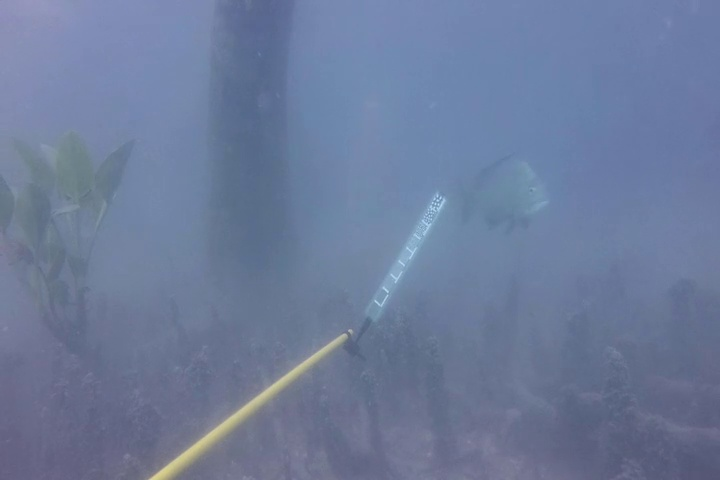
\includegraphics[width=\linewidth]{image/9866/9866_original_frame789.jpg}
            \end{minipage} &
            \begin{minipage}{0.24\textwidth}
                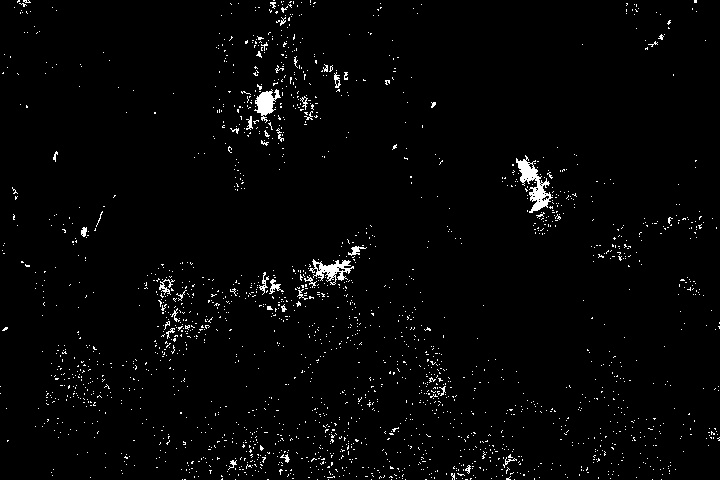
\includegraphics[width=\linewidth]{image/9866/9866_gmm_frame789.jpg}
            \end{minipage} &
            \begin{minipage}{0.24\textwidth}
            	
\includegraphics[width=\linewidth]{image/9866/9866_groundtruth_789.png}
            \end{minipage} &
            8,4 \\ \hline
            849 &
            \begin{minipage}{0.24\textwidth}
                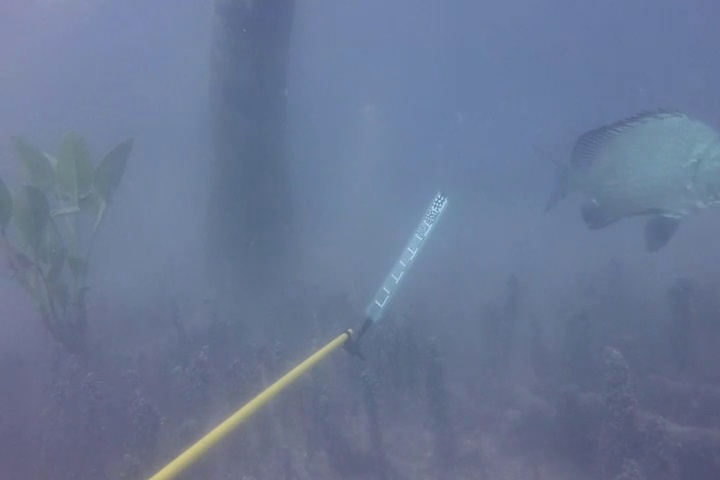
\includegraphics[width=\linewidth]{image/9866/9866_original_frame849.jpg}
            \end{minipage} &
            \begin{minipage}{0.24\textwidth}
                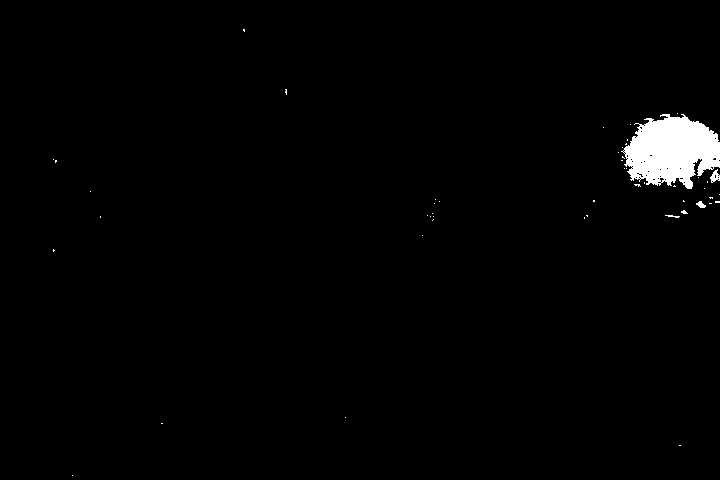
\includegraphics[width=\linewidth]{image/9866/9866_gmm_frame849.jpg}
            \end{minipage} &
            \begin{minipage}{0.24\textwidth}
            	
\includegraphics[width=\linewidth]{image/9866/9866_groundtruth_849.png}
            \end{minipage} &
            44,8 \\ \hline
        \end{longtblr}

        Tabel \ref{tab:gmm_9986} memperlihatkan hasil GMM pada video kategori kedua yaitu, objek tunggal latar belakang kompleks. Dalam pengujian, ketika terdapat \textit{burst of dynamic background} dalam waktu yang singkat (\textit{frame} 789), GMM tampak kesulitan menghasilkan keluaran yang diharapkan, beberapa objek latar belakang yang bergerak \textit{sewaktu-waktu} juga ikut terdeteksi, sehingga menghasilkan skor yang cukup buruk pada frame tersebut.

        \begin{longtblr}[
            caption = {Hasil uji coba proses \textit{background subtraction} menggunakan GMM terhadap video indeks gt\textunderscore124},
            label = {tab:gmm_124}
        ]{
            colspec={|c|c|c|c|c|c|c|},
            rowhead=1
        }
            \hline
            Frame & Citra Asli & Hasil GMM & Groundtruth & \textit{F1} \\ \hline
            705 &
            \begin{minipage}{0.24\textwidth}
                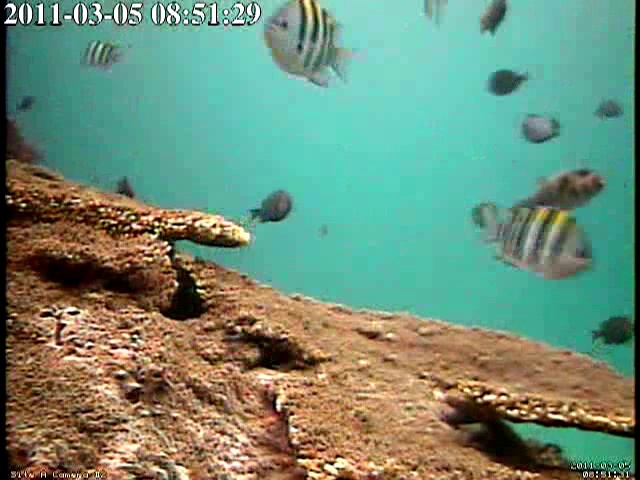
\includegraphics[width=\linewidth]{image/gt_124/gt_124_original_frame705.jpg}
            \end{minipage} &
            \begin{minipage}{0.24\textwidth}
                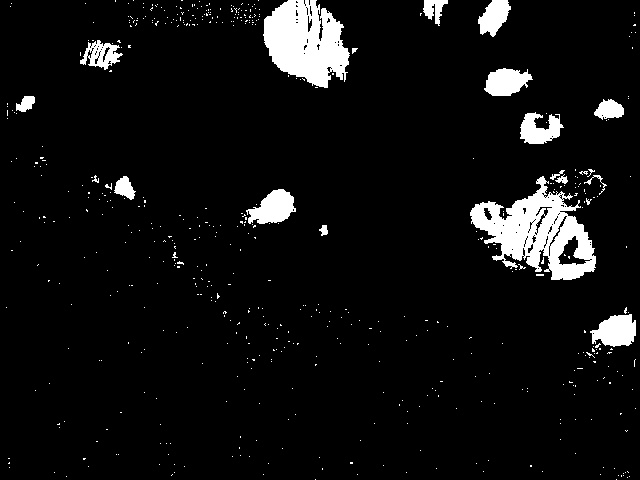
\includegraphics[width=\linewidth]{image/gt_124/gt_124_gmm_frame705.jpg}
            \end{minipage} &
            \begin{minipage}{0.24\textwidth}
            	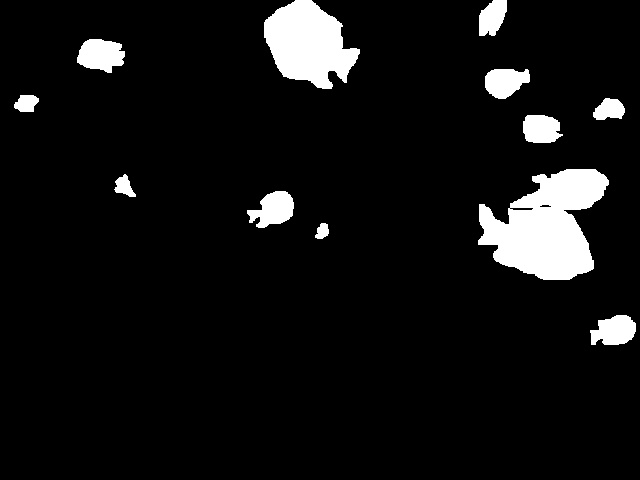
\includegraphics[width=\linewidth]{image/gt_124/gt_124_groundtruth_705.jpg}
            \end{minipage} &
            68,5 \\ \hline
            1173 &
            \begin{minipage}{0.24\textwidth}
                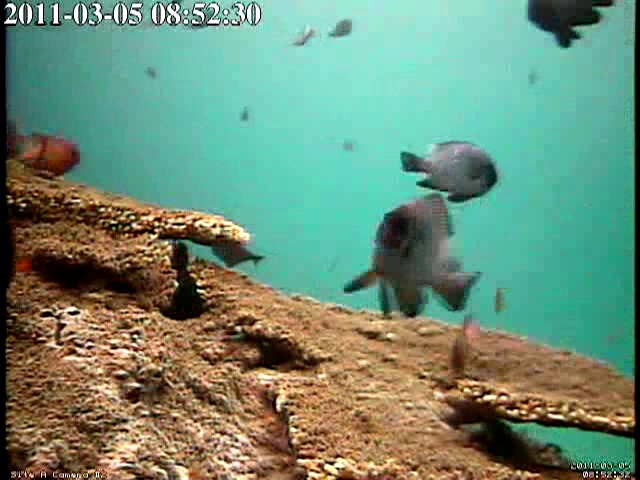
\includegraphics[width=\linewidth]{image/gt_124/gt_124_original_frame1173.jpg}
            \end{minipage} &
            \begin{minipage}{0.24\textwidth}
                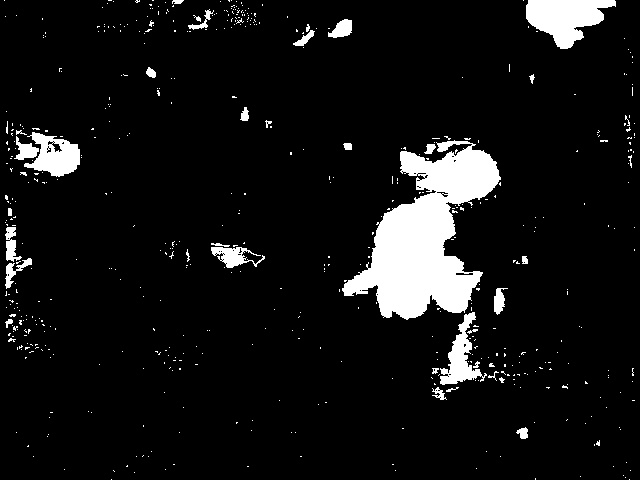
\includegraphics[width=\linewidth]{image/gt_124/gt_124_gmm_frame1173.jpg}
            \end{minipage} &
            \begin{minipage}{0.24\textwidth}
            	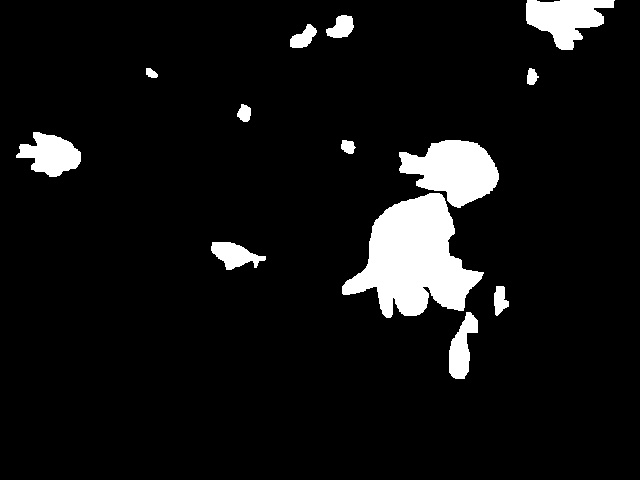
\includegraphics[width=\linewidth]{image/gt_124/gt_124_groundtruth_1173.jpg}
            \end{minipage} &
            80 \\ \hline
            1191 &
            \begin{minipage}{0.24\textwidth}
                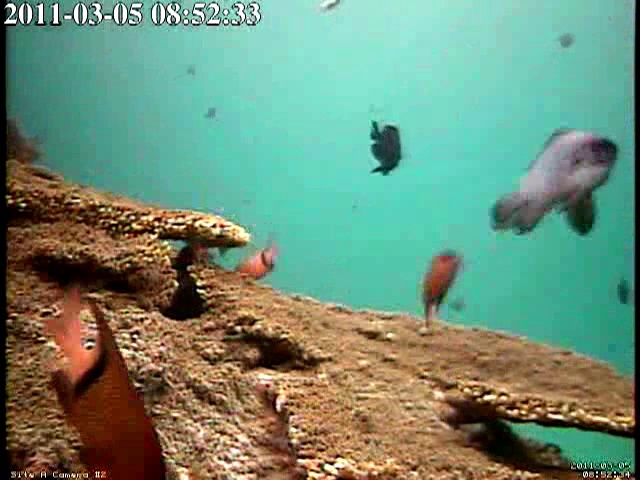
\includegraphics[width=\linewidth]{image/gt_124/gt_124_original_frame1191.jpg}
            \end{minipage} &
            \begin{minipage}{0.24\textwidth}
                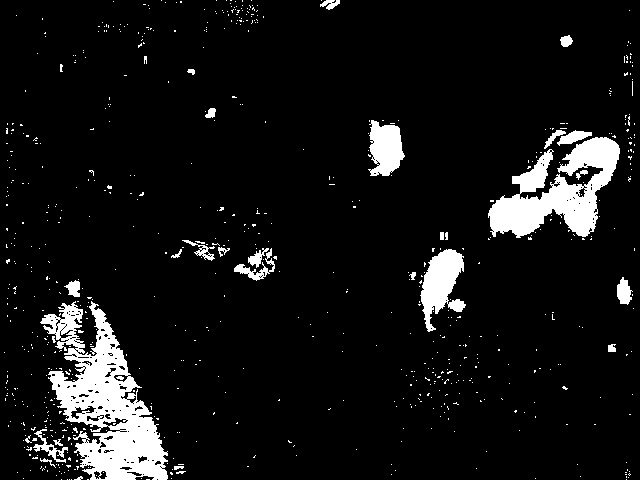
\includegraphics[width=\linewidth]{image/gt_124/gt_124_gmm_frame1191.jpg}
            \end{minipage} &
           \begin{minipage}{0.24\textwidth}
           	
\includegraphics[width=\linewidth]{image/gt_124/gt_124_groundtruth_1191.jpg}
           \end{minipage} &
            67,1 \\ \hline
        \end{longtblr}

        Selanjutnya, GMM dapat menghasilkan keluaran yang cukup baik jika latar belakang video termasuk ke dalam kategori sederhana. Hal ini dapat terlihat pada Tabel \ref{tab:gmm_124} dimana skor tertinggi berada di angka $80\%$, dengan menghasilkan sedikit \textit{noise} yang nantinya akan dieliminasi lebih baik lagi oleh Operasi Morfologi.
        
        Berbeda dengan kasus video indeks gt\textunderscore124, latar belakang pada video indeks gt\textunderscore116 (Tabel \ref{tab:gmm_116}) merupakan latar belakang yang \textit{sangat} dinamis dan kompleks. Dari hasil pengujian, walaupun rata-rata skor yang dihasilkan adalah $58\%$, GMM tampak gagal dalam mengesktrak objek ikan secara keseluruhan. Dikarenakan masih terdapat banyak \textit{noise} latar belakang yang ikut terdeteksi sebagai objek bergerak. Hal ini akan berpengaruh terhadap jumlah objek serta jumlah \textit{track} pada metode-metode selanjutnya, yaitu \textit{Contour Tracing} dan \textit{Kalman Filter}.

        \begin{longtblr}[
            caption = {Hasil uji coba proses \textit{background subtraction} menggunakan GMM terhadap video indeks gt\textunderscore116},
            label = {tab:gmm_116}
        ]{
            colspec={|c|c|c|c|c|c|c|},
            rowhead=1
        }
            \hline
            Frame & Citra Asli & Hasil GMM & Groundtruth & \textit{F1} \\ \hline
            803 &
            \begin{minipage}{0.24\textwidth}
                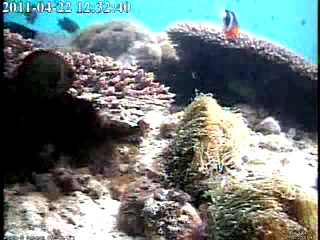
\includegraphics[width=\linewidth]{image/gt_116/gt_116_original_frame803.jpg}
            \end{minipage} &
            \begin{minipage}{0.24\textwidth}
                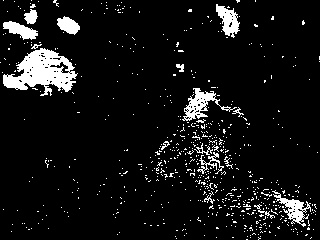
\includegraphics[width=\linewidth]{image/gt_116/gt_116_gmm_frame803.jpg}
            \end{minipage} &
            \begin{minipage}{0.24\textwidth}
            	
\includegraphics[width=\linewidth]{image/gt_116/gt_116_groundtruth_803.jpg}
            \end{minipage} &
            43,5 \\ \hline
            859 &
            \begin{minipage}{0.24\textwidth}
                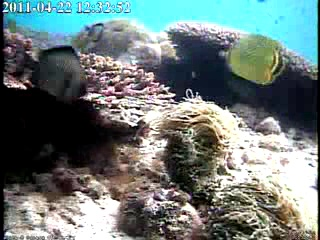
\includegraphics[width=\linewidth]{image/gt_116/gt_116_original_frame859.jpg}
            \end{minipage} &
            \begin{minipage}{0.24\textwidth}
                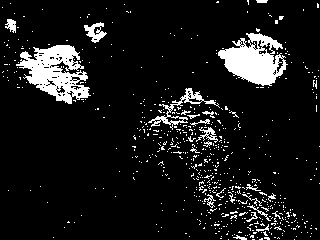
\includegraphics[width=\linewidth]{image/gt_116/gt_116_gmm_frame859.jpg}
            \end{minipage} &
           \begin{minipage}{0.24\textwidth}
           	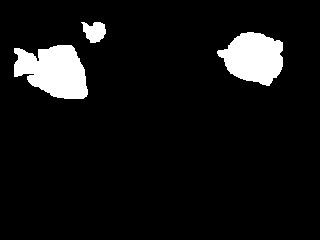
\includegraphics[width=\linewidth]{image/gt_116/gt_116_groundtruth_859.jpg}
           \end{minipage} &
            55,2 \\ \hline
            1167 &
            \begin{minipage}{0.24\textwidth}
                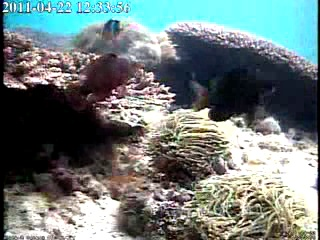
\includegraphics[width=\linewidth]{image/gt_116/gt_116_original_frame1167.jpg}
            \end{minipage} &
            \begin{minipage}{0.24\textwidth}
                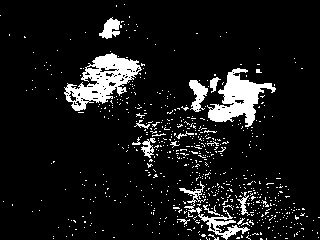
\includegraphics[width=\linewidth]{image/gt_116/gt_116_gmm_frame1167.jpg}
            \end{minipage} &
            \begin{minipage}{0.24\textwidth}
            	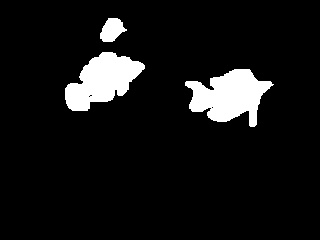
\includegraphics[width=\linewidth]{image/gt_116/gt_116_groundtruth_1167.jpg}
            \end{minipage} &
            50,7 \\ \hline
        \end{longtblr}

        \vspace{-0.5cm}
        \begin{figure}[H]
        \centering
          \singlespacing
          \captionsetup{justification=centering,margin=0.5cm}
          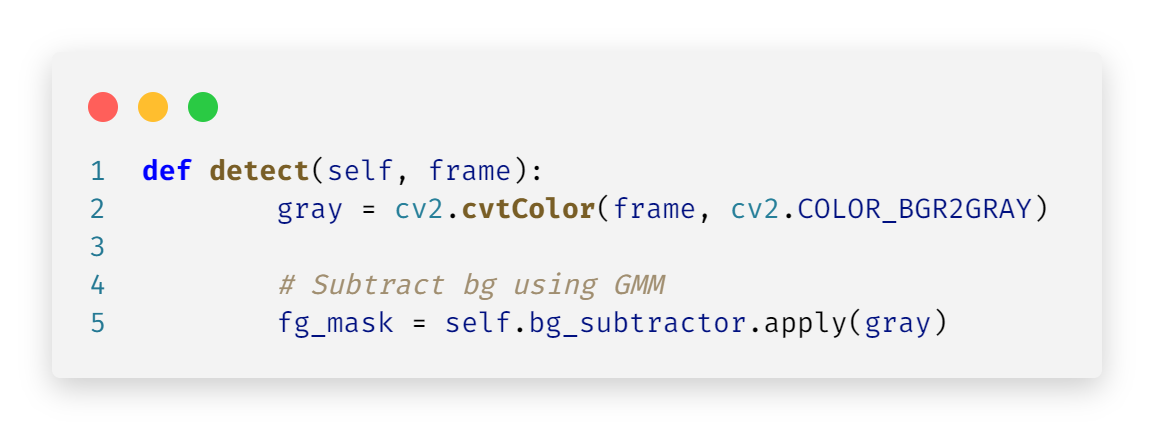
\includegraphics[width=14cm]{image/CodeSnap/gmm.png}
          \caption{Potongan sampel kode Background Subtraction yang dibantu oleh GMM}
          \label{fig:Potongan sampel kode gmm}
        \end{figure}
    
    	\begin{longtblr}[
    		caption = {Skor \textit{Accuracy}, \textit{Recall}, \textit{Precision}, dan \textit{F1} pada metode \textit{Background Subtraction} menggunakan GMM},
    		label = {tab:gmm_skor}
    		]{
    			colspec={|c|c|c|c|c|c|},
    			rowhead=1
    		}
    		\hline
    		Indeks & Frame & \textit{Accuracy} & \textit{Recall} & \textit{Precision} & \textit{F1 Score} \\ \hline
    		9908 &
    		120 &
    		96 &
    		50,3 &
    		68,6 &
    		58 \\ \hline
    		9908 &
    		230 &
    		94,8 &
    		31,9 &
    		31,7 &
    		31,8 \\ \hline
    		9908 &
    		290 &
    		97,2 &
    	    46,9 &
    		77,4 &
    		58,4 \\ \hline
    		9866 &
    		509 &
    		97,5 &
    		27 &
    		91,4 &
    		41,7 \\ \hline
    		9866 &
    		789 &
    		97,6 &
    		9 &
    		7 &
    		8 \\ \hline
    		9866 &
    		849 &
    		96,9 &
    		28,9 &
    		99,4 &
    		44,8 \\ \hline
    		gt\textunderscore124 &
    		705 &
    		96,5 &
    		60,3 &
    		79,2 &
    		68,5 \\ \hline
    		gt\textunderscore124 &
    		1173 &
    		97,4 &
    		79,9 &
    		80,1 &
    		80 \\ \hline
    		gt\textunderscore124 &
    		1191 &
    		95,4 &
    		59,1 &
    		77,7 &
    		67,1 \\ \hline
    		gt\textunderscore116 &
    		803 &
    		94,9 &
    		49,7 &
    		38,6 &
    		43,5 \\ \hline
    		gt\textunderscore116 &
    		859 &
    		94,1 &
    		55,8 &
    		54,9 &
    		55,2 \\ \hline
    		gt\textunderscore116 &
    		1167 &
    		93,6 &
    		49,3 &
    		52,3 &
    		50,7 \\ \hline
    	\end{longtblr}
    
    	Secara teori, GMM seharusnya dapat menghasilkan keluaran yang lebih baik seiring dengan bertambahnya \textit{frame} yang diolah oleh sistem. Dikarenakan proses \textit{training} model latar belakang oleh GMM dapat memanfaatkan jumlah dataset yang lebih banyak. Akan tetapi pada praktiknya, banyak juga faktor yang dapat membuat keluaran metode ini kurang baik. Hasil yang diharapkan adalah skor \textit{Precision} dan \textit{Recall} yang mendekati satu, dimana \textit{Precision} merepresentasikan seberapa besar kasus positif (piksel latar depan) yang benar dari seluruh prediksi positif, dan \textit{Recall} merepresentasikan seberapa besar kasus positif yang benar dari seluruh kasus positif di dataset.
    	
    	Jika dilihat pada Tabel \ref{tab:gmm_skor}, secara garis besar skor GMM cenderung fluktuatif, bahkan dalam beberapa kasus GMM tampak gagal dalam mengekstraksi objek ikan. Contohnya ada pada video indeks 9866 \textit{frame} 789, \textit{F1 Score} menyentuh angka yang sangat rendah, yaitu $8\%$. Hal ini dikarenakan metode mengalami lonjakan input latar belakang dinamis yang sangat besar pada \textit{frame} tersebut. Artinya, model latar belakang yang di-\textit{generate} oleh GMM gagal dalam mengklasifikasikan piksel \textit{frame} ke dalam kelasnya masing-masing.
    	
    	Hal lain yang dapat disimpulkan adalah pada video indeks 9908 dan gt\textunderscore124, dimana kedua dataset tersebut merupakan dataset dengan kategori latar belakang sederhana, menghasilkan rata-rata skor yang lebih tinggi dari pada video indeks 9866 dan gt\textunderscore116, yang merupakan video dengan kategori latar belakang kompleks. Hasil ini seperti yang diharapkan penulis, GMM akan megnhasilkan keluaran yang lebih baik jika sedari awal \textit{noise} yang ada pada masukkan sistem sudah sangat \textit{minim}. Walaupn salah satu fungsi dari GMM itu sendiri adalah mengeliminasi \textit{noise} yang berulang (seperti dahan pohon yang berayun dan iluminasi), akan tetapi jika \textit{noise} itu sendiri sudah tidak ada pada video masukkan tentu hal ini akan berpengaruh terhadap meningkatnya skor yang dihasilkan.
    	
    	\begin{equation}\label{eq:3.5}
    		Precision = \frac{TP}{TP + FP} = \frac{\textit{N. of Correctly Predicted Positive Instances}}{\textit{N. of Total Positive Predictions We Made}}
    	\end{equation}
    
    	\begin{equation}\label{eq:3.5}
	    	Recall = \frac{TP}{TP + FN} = \frac{\textit{N. of Correctly Predicted Positive Instances}}{\textit{N. of Total Positive Instances in the Dataset}}
    	\end{equation}
    
    \vspace{2cm}
        
	\section{Operasi Morfologi}
		Selanjutnya, citra melewati proses eliminasi \textit{noise} menggunakan Operasi Morfologi. Dalam pengujian tahap ini, percobaan dilakukan dengan beberapa nilai \textit{structuring element / kernel} Operasi Morfologi yang berbeda-beda.
  
        \begin{longtblr}[
            caption = {Hasil uji coba proses \textit{background subtraction} menggunakan GMM yang disempurnakan oleh Operasi Morfologi},
            label = {tab:gmm_morph_9908}
        ]{
            colspec={|Q[c,m,1.2cm]|c|c|c|c|},
            rowhead=2
        }
            \hline
            \SetCell[r=2]{} Id / Frame & 
            \SetCell[r=2]{} Hasil GMM &
            \SetCell[c=3]{}{Kernel} \\ \cline{3-5}
            & & $3 \times 9$ & $5 \times 11$ & $7 \times 13$ \\ 
            \hline
            9908 / 120 &
            \begin{minipage}{0.19\textwidth}
                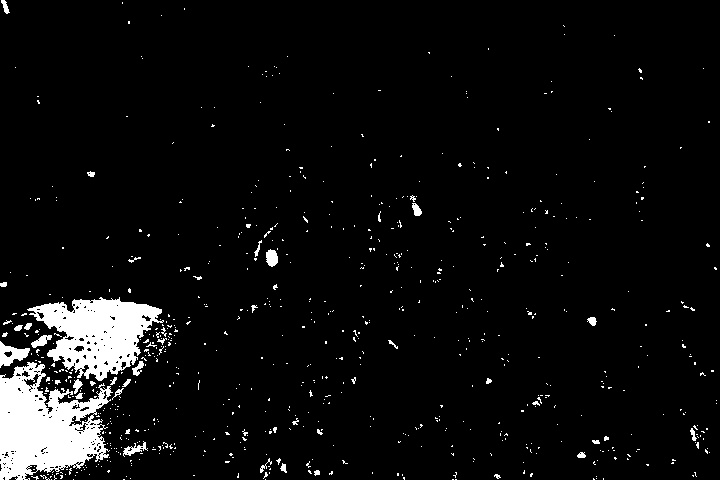
\includegraphics[width=\linewidth]{image/9908/9908_gmm_frame120.jpg}
            \end{minipage} & 
            \begin{minipage}{0.19\textwidth}
                
\includegraphics[width=\linewidth]{image/9908/9908_dilated_3x9_frame120.jpg}
            \end{minipage} &
            \begin{minipage}{0.19\textwidth}
                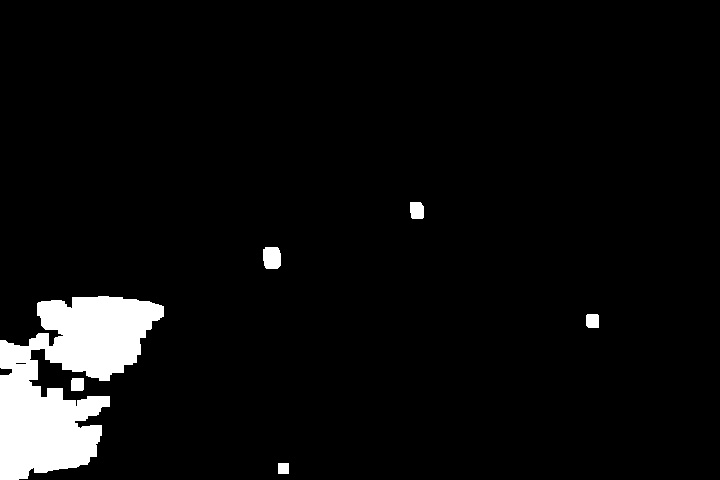
\includegraphics[width=\linewidth]{image/9908/9908_dilated_5x11_frame120.jpg}
            \end{minipage} & 
            \begin{minipage}{0.19\textwidth}
                
\includegraphics[width=\linewidth]{image/9908/9908_dilated_7x13_frame120.jpg}
            \end{minipage} \\
            \hline
            9908 / 230 &
            \begin{minipage}{0.19\textwidth}
                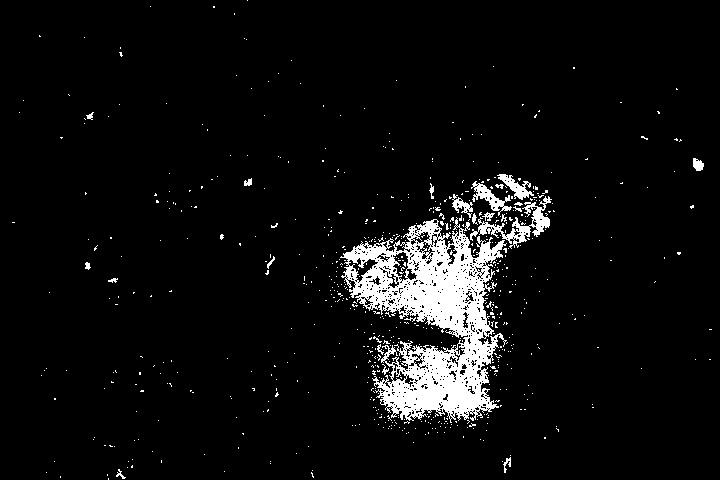
\includegraphics[width=\linewidth]{image/9908/9908_gmm_frame230.jpg}
            \end{minipage} & 
            \begin{minipage}{0.19\textwidth}
                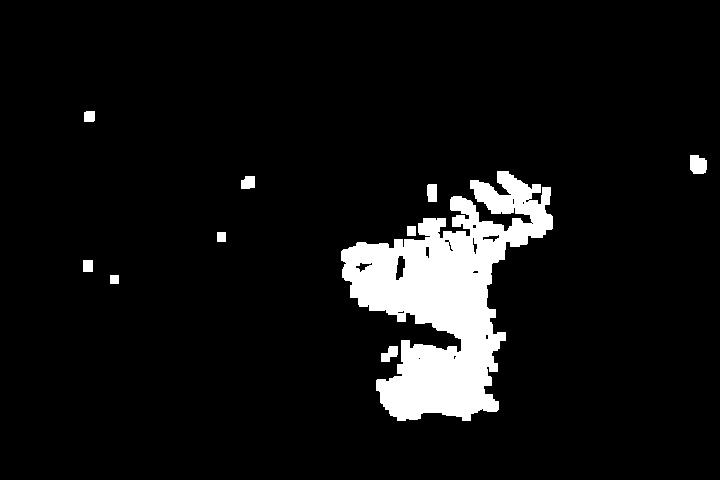
\includegraphics[width=\linewidth]{image/9908/9908_dilated_3x9_frame230.jpg}
            \end{minipage} &
            \begin{minipage}{0.19\textwidth}
                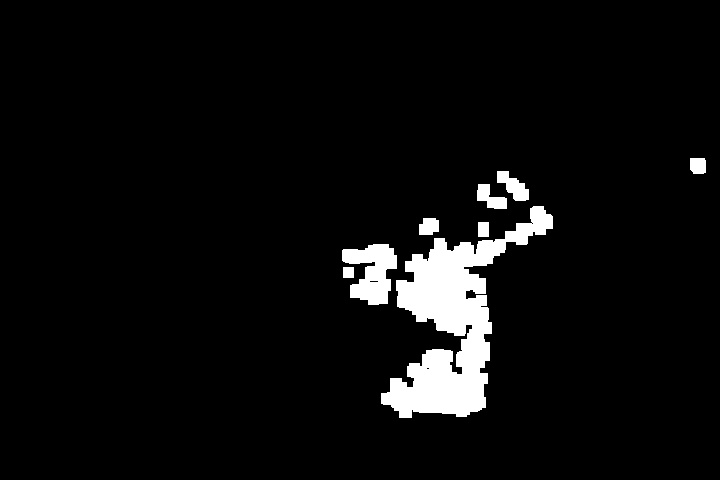
\includegraphics[width=\linewidth]{image/9908/9908_dilated_5x11_frame230.jpg}
            \end{minipage} & 
            \begin{minipage}{0.19\textwidth}
                
\includegraphics[width=\linewidth]{image/9908/9908_dilated_7x13_frame230.jpg}
            \end{minipage} \\
            \hline
            9908 / 290 &
            \begin{minipage}{0.19\textwidth}
                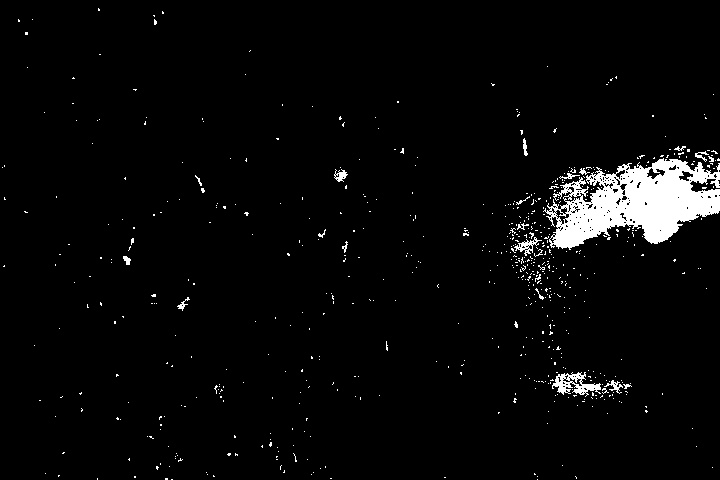
\includegraphics[width=\linewidth]{image/9908/9908_gmm_frame290.jpg}
            \end{minipage} & 
            \begin{minipage}{0.19\textwidth}
                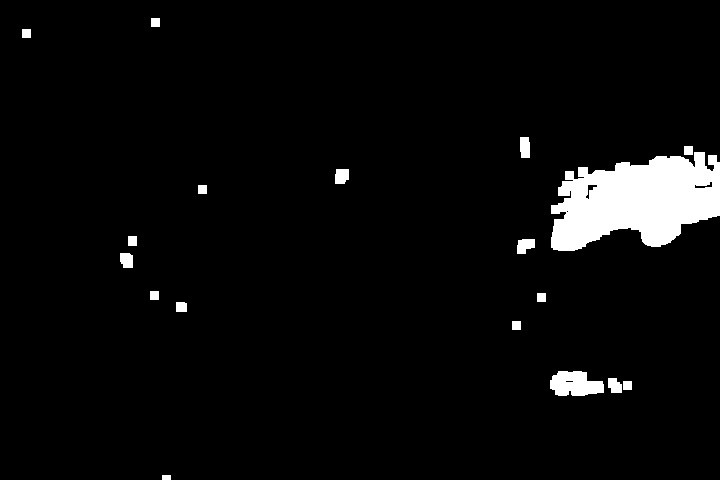
\includegraphics[width=\linewidth]{image/9908/9908_dilated_3x9_frame290.jpg}
            \end{minipage} &
            \begin{minipage}{0.19\textwidth}
                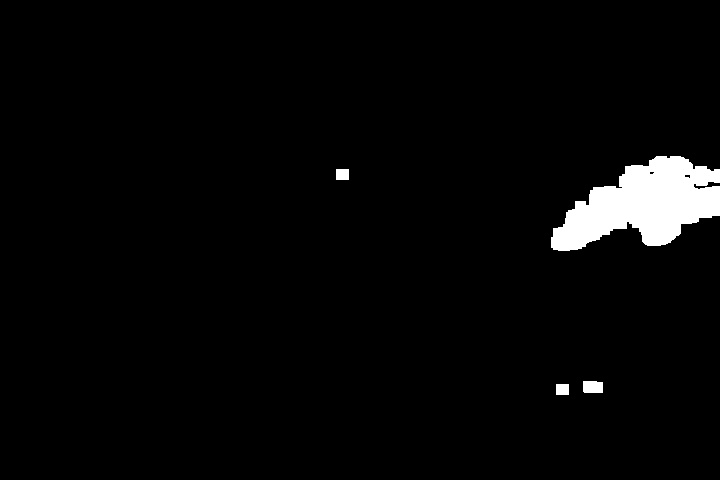
\includegraphics[width=\linewidth]{image/9908/9908_dilated_5x11_frame290.jpg}
            \end{minipage} & 
            \begin{minipage}{0.19\textwidth}
                \includegraphics[width=\linewidth]{image/9908/9908_dilated_7x13_frame290.jpg}
            \end{minipage} \\
            \hline
            9866 / 509 &
            \begin{minipage}{0.19\textwidth}
                \includegraphics[width=\linewidth]{image/9866/9866_gmm_frame509.jpg}
            \end{minipage} & 
            \begin{minipage}{0.19\textwidth}
                \includegraphics[width=\linewidth]{image/9866/9866_dilated_3x9_frame509.jpg}
            \end{minipage} &
            \begin{minipage}{0.19\textwidth}
                \includegraphics[width=\linewidth]{image/9866/9866_dilated_5x11_frame509.jpg}
            \end{minipage} & 
            \begin{minipage}{0.19\textwidth}
                \includegraphics[width=\linewidth]{image/9866/9866_dilated_7x13_frame509.jpg}
            \end{minipage} \\
            \hline
            9866 / 789 &
            \begin{minipage}{0.19\textwidth}
                \includegraphics[width=\linewidth]{image/9866/9866_gmm_frame789.jpg}
            \end{minipage} & 
            \begin{minipage}{0.19\textwidth}
                \includegraphics[width=\linewidth]{image/9866/9866_dilated_3x9_frame789.jpg}
            \end{minipage} &
            \begin{minipage}{0.19\textwidth}
                \includegraphics[width=\linewidth]{image/9866/9866_dilated_5x11_frame789.jpg}
            \end{minipage} & 
            \begin{minipage}{0.19\textwidth}
                \includegraphics[width=\linewidth]{image/9866/9866_dilated_7x13_frame789.jpg}
            \end{minipage} \\
            \hline
            9866 / 849 &
            \begin{minipage}{0.19\textwidth}
                \includegraphics[width=\linewidth]{image/9866/9866_gmm_frame849.jpg}
            \end{minipage} & 
            \begin{minipage}{0.19\textwidth}
                \includegraphics[width=\linewidth]{image/9866/9866_dilated_3x9_frame849.jpg}
            \end{minipage} &
            \begin{minipage}{0.19\textwidth}
                \includegraphics[width=\linewidth]{image/9866/9866_dilated_5x11_frame849.jpg}
            \end{minipage} & 
            \begin{minipage}{0.19\textwidth}
                \includegraphics[width=\linewidth]{image/9866/9866_dilated_7x13_frame849.jpg}
            \end{minipage} \\
            \hline
            gt\textunderscore124 / 705 &
            \begin{minipage}{0.19\textwidth}
                \includegraphics[width=\linewidth]{image/gt_124/gt_124_gmm_frame705.jpg}
            \end{minipage} & 
            \begin{minipage}{0.19\textwidth}
                \includegraphics[width=\linewidth]{image/gt_124/gt_124_dilated_3x9_frame705.jpg}
            \end{minipage} &
            \begin{minipage}{0.19\textwidth}
                \includegraphics[width=\linewidth]{image/gt_124/gt_124_dilated_5x11_frame705.jpg}
            \end{minipage} & 
            \begin{minipage}{0.19\textwidth}
                \includegraphics[width=\linewidth]{image/gt_124/gt_124_dilated_7x13_frame705.jpg}
            \end{minipage} \\
            \hline
            gt\textunderscore124 / 1173 &
            \begin{minipage}{0.19\textwidth}
                \includegraphics[width=\linewidth]{image/gt_124/gt_124_gmm_frame1173.jpg}
            \end{minipage} & 
            \begin{minipage}{0.19\textwidth}
                \includegraphics[width=\linewidth]{image/gt_124/gt_124_dilated_3x9_frame1173.jpg}
            \end{minipage} &
            \begin{minipage}{0.19\textwidth}
                \includegraphics[width=\linewidth]{image/gt_124/gt_124_dilated_5x11_frame1173.jpg}
            \end{minipage} & 
            \begin{minipage}{0.19\textwidth}
                \includegraphics[width=\linewidth]{image/gt_124/gt_124_dilated_7x13_frame1173.jpg}
            \end{minipage} \\
            \hline
            gt\textunderscore124 / 1191 &
            \begin{minipage}{0.19\textwidth}
                \includegraphics[width=\linewidth]{image/gt_124/gt_124_gmm_frame1191.jpg}
            \end{minipage} & 
            \begin{minipage}{0.19\textwidth}
                \includegraphics[width=\linewidth]{image/gt_124/gt_124_dilated_3x9_frame1191.jpg}
            \end{minipage} &
            \begin{minipage}{0.19\textwidth}
                \includegraphics[width=\linewidth]{image/gt_124/gt_124_dilated_5x11_frame1191.jpg}
            \end{minipage} & 
            \begin{minipage}{0.19\textwidth}
                \includegraphics[width=\linewidth]{image/gt_124/gt_124_dilated_7x13_frame1191.jpg}
            \end{minipage} \\
            \hline
            gt\textunderscore116 / 803 &
            \begin{minipage}{0.19\textwidth}
                \includegraphics[width=\linewidth]{image/gt_116/gt_116_gmm_frame803.jpg}
            \end{minipage} & 
            \begin{minipage}{0.19\textwidth}
                \includegraphics[width=\linewidth]{image/gt_116/gt_116_dilated_3x9_frame803.jpg}
            \end{minipage} &
            \begin{minipage}{0.19\textwidth}
                \includegraphics[width=\linewidth]{image/gt_116/gt_116_dilated_5x11_frame803.jpg}
            \end{minipage} & 
            \begin{minipage}{0.19\textwidth}
                \includegraphics[width=\linewidth]{image/gt_116/gt_116_dilated_7x13_frame803.jpg}
            \end{minipage} \\
            \hline
            gt\textunderscore116 / 859 &
            \begin{minipage}{0.19\textwidth}
                \includegraphics[width=\linewidth]{image/gt_116/gt_116_gmm_frame859.jpg}
            \end{minipage} & 
            \begin{minipage}{0.19\textwidth}
                \includegraphics[width=\linewidth]{image/gt_116/gt_116_dilated_3x9_frame859.jpg}
            \end{minipage} &
            \begin{minipage}{0.19\textwidth}
                \includegraphics[width=\linewidth]{image/gt_116/gt_116_dilated_5x11_frame859.jpg}
            \end{minipage} & 
            \begin{minipage}{0.19\textwidth}
                \includegraphics[width=\linewidth]{image/gt_116/gt_116_dilated_7x13_frame859.jpg}
            \end{minipage} \\
            \hline
            gt\textunderscore116 / 1167 &
            \begin{minipage}{0.19\textwidth}
                \includegraphics[width=\linewidth]{image/gt_116/gt_116_gmm_frame1167.jpg}
            \end{minipage} & 
            \begin{minipage}{0.19\textwidth}
                \includegraphics[width=\linewidth]{image/gt_116/gt_116_dilated_3x9_frame1167.jpg}
            \end{minipage} &
            \begin{minipage}{0.19\textwidth}
                \includegraphics[width=\linewidth]{image/gt_116/gt_116_dilated_5x11_frame1167.jpg}
            \end{minipage} & 
            \begin{minipage}{0.19\textwidth}
                \includegraphics[width=\linewidth]{image/gt_116/gt_116_dilated_7x13_frame1167.jpg}
            \end{minipage} \\
            \hline
        \end{longtblr}
    
        Digunakan $3$ parameter \textit{structuring element / kernel} (Operasi Morfologi) untuk masing-masing sampel \textit{frame}. Proses ini menyempurnakan keluaran metode GMM dengan menghapus \textit{noise (noise removal)} secara lebih \textbf{agresif} dan menghasilkan citra biner yang diharapkan bersih dari \textit{noise}. Fokus dari Operasi Morfologi adalah menghapus \textit{noise} sebanyak-banyaknya. Jika dilihat pada Tabel \ref{tab:skor_morph}, skor \textit{metric} cenderung mengalami penurunan seiring dengan semakin besarnya ukuran \textit{kernel} yang digunakan. Hal ini dikarenakan ukuran \textit{kernel} yang lebih besar akan mengikis piksel lebih banyak dari pada ukuran \textit{kernel} yang lebih kecil. Penentuan besaran ukuran \textit{kernel} perlu mempertimbangkan rata-rata ukuran objek yang ingin dilacak untuk meminimalisir piksel objek tereliminasi, atau bahkan dalam kasus terburuk objek tersebut hilang dari \textit{frame}.

        \begin{longtblr}[
            caption = {Skor \textit{Accuracy, Recall, Precision, dan F1} Operasi Morfologi},
            label = {tab:skor_morph}
        ]{
            colspec={|c|c|c|Q[c,m,1.75cm]|Q[c,m,1.75cm]|Q[c,m,1.75cm]|Q[c,m,1.75cm]|},
            rowhead=1
        }
            \hline
            Indeks & Frame & \textit{Kernel} & \textit{Accuracy} & \textit{Recall} & \textit{Precision} & \textit{F1} \\ \hline
            \SetCell[r=3]{} 9908 & \SetCell[r=3]{} 120 & $3 \times 9$ & 96,8 & 78,6 & 68,3 & 73,1 \\ \cline{3-7}
            & & $5 \times 11$ & 97,1 & 68 & 76,1 & 71,8 \\ \cline{3-7}
            & & $7 \times 13$ & 96,8 & 58 & 77,1 & 66,2 \\
            \hline
            \SetCell[r=3]{} 9908 & \SetCell[r=3]{} 230 & $3 \times 9$ & 94,5 & 64,1 & 36,9 & 46,9 \\ \cline{3-7}
            & & $5 \times 11$ & 94,6 & 38,2 & 32,2 & 35 \\ \cline{3-7}
            & & $7 \times 13$ & 94,4 & 12,2 & 16,6 & 14,1 \\
            \hline
            \SetCell[r=3]{} 9908 & \SetCell[r=3]{} 290 & $3 \times 9$ & 97,8 & 70,2 & 76,2 & 73,1 \\ \cline{3-7}
            & & $5 \times 11$ & 97,7 & 57,7 & 88,4 & 69,8 \\ \cline{3-7}
            & & $7 \times 13$ & 97,8 & 51,6 & 92,9 & 66,4 \\
            \hline
            \SetCell[r=3]{} 9866 & \SetCell[r=3]{} 509 & $3 \times 9$ & 97,7 & 44 & 76,8 & 55,9 \\ \cline{3-7}
            & & $5 \times 11$ & 97,5 & 37,4 & 78,1 & 50,5 \\ \cline{3-7}
            & & $7 \times 13$ & 97,4 & 32,7 & 78,5 & 46,2 \\
            \hline
            \SetCell[r=3]{} 9866 & \SetCell[r=3]{} 789 & $3 \times 9$ & 98,1 & 17,5 & 19 & 18,2 \\ \cline{3-7}
            & & $5 \times 11$ & 98,6 & 13,7 & 32,9 & 19,4 \\ \cline{3-7}
            & & $7 \times 13$ & 98,7 & 10,8 & 34,9 & 16,5 \\
            \hline
            \SetCell[r=3]{} 9866 & \SetCell[r=3]{} 849 & $3 \times 9$ & 97,3 & 39,8 & 99 & 56,8 \\ \cline{3-7}
            & & $5 \times 11$ & 97,2 & 36,6 & 99,5 & 53,5 \\ \cline{3-7}
            & & $7 \times 13$ & 97,1 & 34,1 & 99,5 & 50,9 \\
            \hline
            \SetCell[r=1]{} gt\textunderscore124 & \SetCell[r=1]{} 705 & $3 \times 9$ & 96,8 & 86,3 & 69,8  & 77,2 \\ \cline{3-7}
            & & $5 \times 11$ & 96,6 & 80,5 & 70,5 & 75,2 \\ \cline{3-7}
            & & $7 \times 13$ & 96,5 & 74,4 & 71,5 & 72,9 \\
            \hline
            \SetCell[r=3]{} gt\textunderscore124 & \SetCell[r=3]{} 1173 & $3 \times 9$ & 96,5 & 94,6 & 66 & 77,8 \\ \cline{3-7}
            & & $5 \times 11$ & 97,1 & 93 & 71 & 80 \\ \cline{3-7}
            & & $7 \times 13$ & 97,3 & 89,2 & 74,8 & 81,4 \\
            \hline
            \SetCell[r=3]{} gt\textunderscore124 & \SetCell[r=3]{} 1191 & $3 \times 9$ & 96,3 & 90,9 & 70,5 & 79,4 \\ \cline{3-7}
            & & $5 \times 11$ & 96,6 & 81,7 & 76,1 & 78,8 \\ \cline{3-7}
            & & $7 \times 13$ & 96,2 & 71,4 & 77,74 & 74,3 \\
            \hline
            \SetCell[r=3]{} gt\textunderscore116 & \SetCell[r=3]{} 803 & $3 \times 9$ & 95 & 85,1 & 43,3 & 57,4 \\ \cline{3-7}
            & & $5 \times 11$ & 96,1 & 76,8 & 50,7 & 61,1 \\ \cline{3-7}
            & & $7 \times 13$ & 96,8 & 65,3 & 59,6 & 62,3 \\
            \hline
            \SetCell[r=3]{} gt\textunderscore116 & \SetCell[r=3]{} 859 & $3 \times 9$ & 95,2 & 89,7 & 58,1 & 70,5 \\ \cline{3-7}
            & & $5 \times 11$ & 96, & 72,6 & 69,3 & 70,9 \\ \cline{3-7}
            & & $7 \times 13$ & 96,2 & 58,5 & 77,2 & 66,6 \\
            \hline
            \SetCell[r=3]{} gt\textunderscore116 & \SetCell[r=3]{} 1167 & $3 \times 9$ & 94,8 & 85, & 57,6 & 68,7 \\ \cline{3-7}
            & & $5 \times 11$ & 96,2 & 72,9 & 71,1 & 72 \\ \cline{3-7}
            & & $7 \times 13$ & 96 & 58,5 & 76 & 66 \\
            \hline
            
        \end{longtblr}

        Penentuan 2 besaran ukuran \textit{kernel} yang digunakan, juga mempertimbangkan \textit{trade-off} yang dihasilkan dari masing-masing parameter tersebut. Semakin besar ukuran \textit{kernel}, semakin sedikit \textit{noise} yang tampak, akan tetapi semakin banyak juga informasi yang hilang (piksel objek). Hal ini berdampak pada ukuran serta bentuk objek yang juga ikut menyusut. Sebaliknya, semakin kecil ukuran \textit{kernel} yang digunakan, maka semakin banyak informasi (piksel objek) yang dapat dipertahankan, namun semakin banyak juga \textit{noise} yang tampak. Hasil skor keluaran Operasi Morfologi dapat dilihat pada Tabel \ref{tab:skor_morph}. 
        
        \vspace{-0.5cm}
        \begin{figure}[H]
        \centering
          \singlespacing
          \captionsetup{justification=centering,margin=0.5cm}
          \includegraphics[width=10cm]{image/CodeSnap/morph.png}
          \caption{Potongan sampel kode \textit{Background Subtraction} dan Operasi Morfologi}
          \label{fig:code_gmm_morph}
        \end{figure}
    
    	Dari ujicoba di atas, dapat disimpulkan bahwa secara visual metode ini melaksanakan tugasnya dengan baik, yaitu mengeliminasi \textit{noise} dengan lebih agresif. Pada setiap \textit{frame} uji Tabel \ref{tab:gmm_morph_9908}, \textit{salt and peper noise} dapat dieliminasi dengan baik untuk semua ukuran \textit{structuring element} yang digunakan. Poin penting lain yang dapat diobservasi adalah skor metode yang tampak menurun seiring dengan besarnya ukuran \textit{structuring element} yang digunakan (Tabel \ref{tab:skor_morph}). Hal ini masih masuk ke dalam ekspektasi penulis dikarenakan penjelasan dari metode itu sendiri, dimana \textit{trade-off} yang dihasilkan dari semakin besarnya ukuran \textit{structuring element} yang digunakan, adalah semakin banyak piksel latar depan yang hilang, akan tetapi semakin banyak juga \textit{noise} yang tereliminasi.
    	
    	Metode ini hanya berfokus terhadap seberapa banyak \textit{noise} yang dapat dieliminasi dengan tetap mempertahankan bentuk objek sebaik mungkin. Maka dari itu, skor \textit{metric} yang semakin menurun bukan semata-mata pertanda bahwa performa sistem buruk, semua bergantung pada hasil metode selanjutnya, yaitu \textit{Contour Tracing} dan \textit{Kalman Filter} yang akan memvalidasi jumlah objek hasil deteksi, agar \textit{noise} yang dihasilkan GMM tidak ikut terhitung oleh metode tersebut.

    \section{\textit{Contour Tracing} dan \textit{Downsampling}}
        Pada uji coba CT, setiap \textit{frame} data diuji dengan skala \textit{Downsampling} yang berbeda-beda. Hal ini akan berpengaruh terhadap performa metode CT. Semakin besar skala yang digunakan, maka semakin cepat performa yang didapat, begitu juga sebaliknya. Pemilihan besaran skala \textit{Downsampling} juga tetap memperhatikan hasil \textit{bounding box} dari metode CT tersebut.
        
        \begin{longtblr}[
            caption = {Hasil uji coba metode CT yang ditingkatkan oleh \textit{Downsampling} pada video indeks 9908 dengan ukuran \textit{kernel} Operasi Morfologi 7x13},
            label = {tab:ct_downsampling_9908}
        ]{
            colspec={|c|c|c|c|c|},
            rowhead=1
        }
            \hline
            Indeks & Frame & \textit{Groundtruth} & Skala & Hasil \\ 
            \hline
            % row
            \SetCell[r=3]{} 9908 &
            \SetCell[r=3]{} 120 &
            \SetCell[r=3]{} \begin{minipage}{0.3\textwidth}
                \includegraphics[width=\linewidth]{image/9908/9908_groundtruth_120.png}
            \end{minipage} &
            $\times2$ & 
            \begin{minipage}{0.3\textwidth}
                \includegraphics[width=\linewidth]{image/9908/9908_contour_downsample_x2_m7x13_frame120.jpg}
            \end{minipage} \\ \cline{3-4}
            & & & 
            $\times4$ &
            \begin{minipage}{0.3\textwidth}
                \includegraphics[width=\linewidth]{image/9908/9908_contour_downsample_x4_m7x13_frame120.jpg}
            \end{minipage} \\ \cline{3-4}
            & & & 
            $\times8$ &
            \begin{minipage}{0.3\textwidth}
                \includegraphics[width=\linewidth]{image/9908/9908_contour_downsample_x8_m7x13_frame120.jpg}
            \end{minipage} \\ 
            \hline
            % end row
            % row
            \SetCell[r=3]{} 9908 &
            \SetCell[r=3]{} 230 &
            \SetCell[r=3]{} \begin{minipage}{0.3\textwidth}
                \includegraphics[width=\linewidth]{image/9908/9908_groundtruth_230.png}
            \end{minipage} &
            $\times2$ & 
            \begin{minipage}{0.3\textwidth}
                \includegraphics[width=\linewidth]{image/9908/9908_contour_downsample_x2_m7x13_frame230.jpg}
            \end{minipage} \\ \cline{3-4}
            & & \SetCell[r=2]{} &
            $\times4$ &
            \begin{minipage}{0.3\textwidth}
                \includegraphics[width=\linewidth]{image/9908/9908_contour_downsample_x4_m7x13_frame230.jpg}
            \end{minipage} \\ \cline{3-4}
            & & &
            $\times8$ &
            \begin{minipage}{0.3\textwidth}
                \includegraphics[width=\linewidth]{image/9908/9908_contour_downsample_x8_m7x13_frame230.jpg}
            \end{minipage} \\ 
            \hline
            % end row
            % row
            \SetCell[r=3]{} 9908 &
            \SetCell[r=3]{} 290 &
            \SetCell[r=3]{} \begin{minipage}{0.3\textwidth}
                \includegraphics[width=\linewidth]{image/9908/9908_groundtruth_290.png}
            \end{minipage} &
            $\times2$ & 
            \begin{minipage}{0.3\textwidth}
                \includegraphics[width=\linewidth]{image/9908/9908_contour_downsample_x2_m7x13_frame290.jpg}
            \end{minipage} \\ \cline{3-4}
            & & & 
            $\times4$ &
            \begin{minipage}{0.3\textwidth}
                \includegraphics[width=\linewidth]{image/9908/9908_contour_downsample_x4_m7x13_frame290.jpg}
            \end{minipage} \\ \cline{3-4}
            & & & 
            $\times8$ &
            \begin{minipage}{0.3\textwidth}
                \includegraphics[width=\linewidth]{image/9908/9908_contour_downsample_x8_m7x13_frame290.jpg}
            \end{minipage} \\ 
            \hline
            % end row
        \end{longtblr}

        \begin{longtblr}[
            caption = {Hasil uji coba metode CT yang ditingkatkan oleh \textit{Downsampling} pada video indeks 9866 dengan ukuran \textit{Kernel} Operasi Morfologi 7x13},
            label = {tab:ct_downsampling_9866}
        ]{
            colspec={|c|c|c|c|c|},
            rowhead=1
        }
            \hline
            Indeks & Frame & \textit{Groundtruth} & Skala & Hasil \\ 
            \hline
            % row
            \SetCell[r=3]{} 9866 &
            \SetCell[r=3]{} 509 &
            \SetCell[r=3]{} \begin{minipage}{0.3\textwidth}
                \includegraphics[width=\linewidth]{image/9866/9866_groundtruth_509.png}
            \end{minipage} &
            $\times2$ & 
            \begin{minipage}{0.3\textwidth}
                \includegraphics[width=\linewidth]{image/9866/9866_contour_downsample_x2_m7x13_frame509.jpg}
            \end{minipage} \\ \cline{3-4}
            & & & 
            $\times4$ &
            \begin{minipage}{0.3\textwidth}
                \includegraphics[width=\linewidth]{image/9866/9866_contour_downsample_x4_m7x13_frame509.jpg}
            \end{minipage} \\ \cline{3-4}
            & & & 
            $\times8$ &
            \begin{minipage}{0.3\textwidth}
                \includegraphics[width=\linewidth]{image/9866/9866_contour_downsample_x8_m7x13_frame509.jpg}
            \end{minipage} \\ 
            \hline
            % end row
            % row
            \SetCell[r=1]{} 9866 &
            \SetCell[r=1]{} 789 &
            \SetCell[r=1]{} \begin{minipage}{0.3\textwidth}
                \includegraphics[width=\linewidth]{image/9866/9866_groundtruth_789.png}
            \end{minipage} &
            $\times2$ & 
            \begin{minipage}{0.3\textwidth}
                \includegraphics[width=\linewidth]{image/9866/9866_contour_downsample_x2_m7x13_frame789.jpg}
            \end{minipage} \\ \cline{3-4}
            & & &
            $\times4$ &
            \begin{minipage}{0.3\textwidth}
                \includegraphics[width=\linewidth]{image/9866/9866_contour_downsample_x4_m7x13_frame789.jpg}
            \end{minipage} \\ \cline{4-4}
            & & &
            $\times8$ &
            \begin{minipage}{0.3\textwidth}
                \includegraphics[width=\linewidth]{image/9866/9866_contour_downsample_x8_m7x13_frame789.jpg}
            \end{minipage} \\ 
            \hline
            % end row
            % row
            \SetCell[r=3]{} 9866 &
            \SetCell[r=3]{} 849 &
            \SetCell[r=3]{} \begin{minipage}{0.3\textwidth}
                \includegraphics[width=\linewidth]{image/9866/9866_groundtruth_849.png}
            \end{minipage} &
            $\times2$ & 
            \begin{minipage}{0.3\textwidth}
                \includegraphics[width=\linewidth]{image/9866/9866_contour_downsample_x2_m7x13_frame849.jpg}
            \end{minipage} \\ \cline{3-4}
            & & & 
            $\times4$ &
            \begin{minipage}{0.3\textwidth}
                \includegraphics[width=\linewidth]{image/9866/9866_contour_downsample_x4_m7x13_frame849.jpg}
            \end{minipage} \\ \cline{3-4}
            & & & 
            $\times8$ &
            \begin{minipage}{0.3\textwidth}
                \includegraphics[width=\linewidth]{image/9866/9866_contour_downsample_x8_m7x13_frame849.jpg}
            \end{minipage} \\ 
            \hline
            % end row
        \end{longtblr}
    
    	Pada Tabel \ref{tab:ct_downsampling_9908} dan Tabel \ref{tab:ct_downsampling_9866}, setiap dataset uji \textit{(frame)} dibandingkan terhadap \textit{groundtruth}-nya masing-masing. Dapat diperhatikan bahwa tidak terdapat perbedaan \textit{bounding box} yang cukup signifikan untuk setiap skala yang digunakan. \textit{Bounding box} hanya tampak sedikit bergeser seiring dengan membesarnya skala \textit{Downsampling} tersebut. Maka dari itu, penggunaan skala yang besar sangat setimpal dengan performa yang dihasilkan, dikarenakan semakin besar skala yang digunanakn, akan semakin cepat juga metode CT berjalan. 
    	
    	Hal yang sama juga akan ditemukan pada Tabel \ref{tab:ct_downsampling_gt_124} dan Tabel \ref{tab:ct_downsampling_gt_116}. Pengujian metode CT berfokus pada kecepatan serta keberhasilan metode dalam melacak \textit{contour} masing-masing objek. Terkait jumlah objek yang tampak, sepenuhnya bergantung kepada metode sebelumnya, yaitu \textit{background subtraction} menggunaakn GMM yang disempurnakan oleh Operasi Morfologi. Walaupun dalam praktiknya, selisih jumlah objek juga dapat terjadi akibat penggunaan skala \textit{downsampling} yang berbeda-beda (lihat Tabel\ref{tab:ct_score}).
        
        \begin{longtblr}[
            caption = {Hasil uji coba metode CT yang ditingkatkan oleh \textit{Downsampling} pada video indeks gt\textunderscore124 dengan ukuran \textit{kernel} Operasi Morfologi 7x13},
            label = {tab:ct_downsampling_gt_124}
        ]{
            colspec={|c|c|c|c|c|},
            rowhead=1
        }
            \hline
            Indeks & Frame & \textit{Groundtruth} & Skala & Hasil \\ 
            \hline
            % row
            \SetCell[r=3]{} gt\textunderscore124 &
            \SetCell[r=3]{} 705 &
            \SetCell[r=3]{} \begin{minipage}{0.3\textwidth}
                \includegraphics[width=\linewidth]{image/gt_124/gt_124_groundtruth_705.jpg}
            \end{minipage} &
            $\times2$ & 
            \begin{minipage}{0.3\textwidth}
                \includegraphics[width=\linewidth]{image/gt_124/gt_124_contour_downsample_x2_m7x13_frame705.jpg}
            \end{minipage} \\ \cline{3-4}
            & & & 
            $\times4$ &
            \begin{minipage}{0.3\textwidth}
                \includegraphics[width=\linewidth]{image/gt_124/gt_124_contour_downsample_x4_m7x13_frame705.jpg}
            \end{minipage} \\ \cline{3-4}
            & & & 
            $\times8$ &
            \begin{minipage}{0.3\textwidth}
                \includegraphics[width=\linewidth]{image/gt_124/gt_124_contour_downsample_x8_m7x13_frame705.jpg}
            \end{minipage} \\ 
            \hline
            % end row
            % row
            \SetCell[r=3]{} gt\textunderscore124 &
            \SetCell[r=3]{} 1173 &
            \SetCell[r=3]{} \begin{minipage}{0.3\textwidth}
                \includegraphics[width=\linewidth]{image/gt_124/gt_124_groundtruth_1173.jpg}
            \end{minipage} &
            $\times2$ & 
            \begin{minipage}{0.3\textwidth}
                \includegraphics[width=\linewidth]{image/gt_124/gt_124_contour_downsample_x2_m7x13_frame1173.jpg}
            \end{minipage} \\ \cline{3-4}
            & & &
            $\times4$ &
            \begin{minipage}{0.3\textwidth}
                \includegraphics[width=\linewidth]{image/gt_124/gt_124_contour_downsample_x4_m7x13_frame1173.jpg}
            \end{minipage} \\ \cline{3-4}
            & & &
            $\times8$ &
            \begin{minipage}{0.3\textwidth}
                \includegraphics[width=\linewidth]{image/gt_124/gt_124_contour_downsample_x8_m7x13_frame1173.jpg}
            \end{minipage} \\ 
            \hline
            % end row
            % row
            \SetCell[r=3]{} gt\textunderscore124 &
            \SetCell[r=3]{} 1191 &
            \SetCell[r=3]{} \begin{minipage}{0.3\textwidth}
                \includegraphics[width=\linewidth]{image/gt_124/gt_124_groundtruth_1191.jpg}
            \end{minipage} &
            $\times2$ & 
            \begin{minipage}{0.3\textwidth}
                \includegraphics[width=\linewidth]{image/gt_124/gt_124_contour_downsample_x2_m7x13_frame1191.jpg}
            \end{minipage} \\ \cline{3-4}
            & & & 
            $\times4$ &
            \begin{minipage}{0.3\textwidth}
                \includegraphics[width=\linewidth]{image/gt_124/gt_124_contour_downsample_x4_m7x13_frame1191.jpg}
            \end{minipage} \\ \cline{3-4}
            & & & 
            $\times8$ &
            \begin{minipage}{0.3\textwidth}
                \includegraphics[width=\linewidth]{image/gt_124/gt_124_contour_downsample_x8_m7x13_frame1191.jpg}
            \end{minipage} \\ 
            \hline
            % end row
        \end{longtblr}
    
   		Performa metode CT akan benar-bernar diuji ketika citra masukan berasal dari video kategori ke-3 dan ke-4, yaitu video dengan objek lebih dari satu. Proses \textit{contour tracing} yang penulis implementasi memiliki kompleksitas yang cukup tinggi. Semakin banyak objek yang perlu di-\textit{tracing} dalam setiap \textit{frame}, semakin besar juga waktu yang dibutuhkan sistem untuk menyelesaikan hal tersebut. Maka dari itu, diperlukanlah metode \textit{Downsampling} yang dapat mempercepat performa metode CT tanpa merusak citra yang sudah ada. Digunakan skala $\times2, \times4, \text{dan} \times8$ terhadap masing-masing citra keluaran metode sebelumnya.
        
        \begin{longtblr}[
            caption = {Hasil uji coba performa metode CT yang ditingkatkan oleh \textit{Downsampling} pada video indeks gt\textunderscore116 dengan ukuran \textit{kernel} Operasi Morfologi 7x13},
            label = {tab:ct_downsampling_gt_116}
        ]{
            colspec={|c|c|c|c|c|},
            rowhead=1
        }
            \hline
            Indeks & Frame & \textit{Groundtruth} & Skala & Hasil \\ 
            \hline
            % row
            \SetCell[r=3]{} gt\textunderscore116 &
            \SetCell[r=3]{} 803 &
            \SetCell[r=3]{} \begin{minipage}{0.3\textwidth}
                \includegraphics[width=\linewidth]{image/gt_116/gt_116_groundtruth_803.jpg}
            \end{minipage} &
            $\times2$ & 
            \begin{minipage}{0.3\textwidth}
                \includegraphics[width=\linewidth]{image/gt_116/gt_116_contour_downsample_x2_m7x13_frame803.jpg}
            \end{minipage} \\ \cline{3-4}
            & & & 
            $\times4$ &
            \begin{minipage}{0.3\textwidth}
                \includegraphics[width=\linewidth]{image/gt_116/gt_116_contour_downsample_x4_m7x13_frame803.jpg}
            \end{minipage} \\ \cline{3-4}
            & & & 
            $\times8$ &
            \begin{minipage}{0.3\textwidth}
                \includegraphics[width=\linewidth]{image/gt_116/gt_116_contour_downsample_x8_m7x13_frame803.jpg}
            \end{minipage} \\ 
            \hline
            % end row
            % row
            \SetCell[r=3]{} gt\textunderscore116 &
            \SetCell[r=3]{} 859 &
            \SetCell[r=3]{} \begin{minipage}{0.3\textwidth}
                \includegraphics[width=\linewidth]{image/gt_116/gt_116_groundtruth_859.jpg}
            \end{minipage} &
            $\times2$ & 
            \begin{minipage}{0.3\textwidth}
                \includegraphics[width=\linewidth]{image/gt_116/gt_116_contour_downsample_x2_m7x13_frame859.jpg}
            \end{minipage} \\ \cline{3-4}
            & & &
            $\times4$ &
            \begin{minipage}{0.3\textwidth}
                \includegraphics[width=\linewidth]{image/gt_116/gt_116_contour_downsample_x4_m7x13_frame859.jpg}
            \end{minipage} \\ \cline{3-4}
            & & &
            $\times8$ &
            \begin{minipage}{0.3\textwidth}
                \includegraphics[width=\linewidth]{image/gt_116/gt_116_contour_downsample_x8_m7x13_frame859.jpg}
            \end{minipage} \\ 
            \hline
            % end row
            % row
            \SetCell[r=3]{} gt\textunderscore116 &
            \SetCell[r=3]{} 1167 &
            \SetCell[r=3]{} \begin{minipage}{0.3\textwidth}
                \includegraphics[width=\linewidth]{image/gt_116/gt_116_groundtruth_1167.jpg}
            \end{minipage} &
            $\times2$ & 
            \begin{minipage}{0.3\textwidth}
                \includegraphics[width=\linewidth]{image/gt_116/gt_116_contour_downsample_x2_m7x13_frame1167.jpg}
            \end{minipage} \\ \cline{3-4}
            & & & 
            $\times4$ &
            \begin{minipage}{0.3\textwidth}
                \includegraphics[width=\linewidth]{image/gt_116/gt_116_contour_downsample_x4_m7x13_frame1167.jpg}
            \end{minipage} \\ \cline{3-4}
            & & & 
            $\times8$ &
            \begin{minipage}{0.3\textwidth}
                \includegraphics[width=\linewidth]{image/gt_116/gt_116_contour_downsample_x8_m7x13_frame859.jpg}
            \end{minipage} \\ 
            \hline
            % end row
        \end{longtblr}
    
    	Tabel \ref{tab:ct_single_score} dan Tabel \ref{tab:ct_multiple_score} memperlihatkan evaluasi performa metode CT terhadap ukuran \textit{kernel} morfologi dan skala \textit{Downsampling} yang berbeda-beda. Kolom "Waktu" merepresentasikan waktu eksekusi metode CT dalam detik, kolom "Jumlah" merepresentasikan jumlah tepi objek yang berhasil diekstrak, kolom "Jumlah Sebenarnya" merepresentasikan jumlah objek sebenarnya dari citra \textit{groundtruth}, sementara kolom \textit{"Selisih"} merepresentasikan selisih nilai antara kalkulasi jumlah hasil CT dengan jumlah sebenarnya.
    
	    \begin{longtblr}[
	    	caption = {Evaluasi hasil dan performa metode CT video kategori objek tunggal terhadap ukuran \textit{kernel} Operasi Morofologi serta skala \textit{Downsampling} yang berbeda-beda},
	    	label = {tab:ct_single_score}
	    	]{
	    		colspec={|c|c|c|c|c|c|Q[c,m,2cm]|c|},
	    		rowhead=1
	    	}
    		\hline
	    	Indeks & Frame & \textit{Kernel} & Skala & Waktu & Jumlah & Jumlah Sebenarnya & Selisih \\
	    	\hline
	    	\SetCell[r=9]{} 9908 & \SetCell[r=9]{} 120  & \SetCell[r=3]{} $3\times9$  & $\times2$ & 0,28 & 36 & 1 & 35 \\ \cline{4-8} 
						    	 &                      &                       	  & $\times4$ & 0,07 & 34 & 1 & 33 \\ \cline{4-8} 
						    	 &                      &                       	  & $\times8$ & 0,01 & 30 & 1 & 29 \\ \cline{3-8} 
						    	 &                      & \SetCell[r=3]{} $5\times11$ & $\times2$ & 0,26 & 6 & 1 & 5 \\ \cline{4-8} 
						    	 &                      &                       	  & $\times4$ & 0,07 & 6 & 1 & 5 \\ \cline{4-8} 
						       	 &                      &                       	  & $\times8$ & 0,02 & 6 & 1 & 5 \\ \cline{3-8} 
						    	 &                      & \SetCell[r=3]{} $7\times13$ & $\times2$ & 0,39 & 6 & 1 & 5 \\ \cline{4-8} 
						     	 &                      &                       	  & $\times4$ & 0,07 & 5 & 1 & 4 \\ \cline{4-8} 
						    	 &                      &                       	  & $\times8$ & 0,01 & 5 & 1 & 4 \\ \hline
    	 	\SetCell[r=3]{} 9908 & \SetCell[r=3]{} 230  & \SetCell[r=3]{} $3\times9$  & $\times2$ & 0,22 & 25 & 1 & 24  \\ \cline{4-8} 
						    	 &                      &                       	  & $\times4$ & 0,06 & 16 & 1 & 15  \\ \cline{4-8} 
						    	 &                      &                       	  & $\times8$ & 0,01 & 14 & 1 & 13  \\ \cline{3-8} 
						    	 &                      & \SetCell[r=3]{} $5\times11$ & $\times2$ & 0,24 & 10 & 1 & 9 \\ \cline{4-8} 
						    	 &                      &                       	  & $\times4$ & 0,1 & 10 & 1 & 9 \\ \cline{4-8} 
						    	 &                      &                       	  & $\times8$ & 0,02 & 7 & 1 & 6 \\ \cline{3-8} 
						    	 &                      & \SetCell[r=3]{} $7\times13$ & $\times2$ & 0,28 & 9 & 1 & 8 \\ \cline{4-8} 
						    	 &                      &                       	  & $\times4$ & 0,08 & 8 & 1 & 7 \\ \cline{4-8} 
						    	 &                      &                       	  & $\times8$ & 0,02 & 9 & 1 & 8 \\ \hline
    		\SetCell[r=9]{} 9908 & \SetCell[r=9]{} 290  & \SetCell[r=3]{} $3\times9$  & $\times2$ & 0,23 & 22 & 1 & 21 \\ \cline{4-8} 
						    	 &                      &                       	  & $\times4$ & 0,05 & 21 & 1 & 20 \\ \cline{4-8} 
						    	 &                      &                       	  & $\times8$ & 0,01 & 15 & 1 & 14 \\ \cline{3-8} 
						    	 &                      & \SetCell[r=3]{} $5\times11$ & $\times2$ & 0,39 & 7 & 1 & 6 \\ \cline{4-8} 
						    	 &                      &                       	  & $\times4$ & 0,07 & 5 & 1 & 4 \\ \cline{4-8} 
						    	 &                      &                       	  & $\times8$ & 0,07 & 4 & 1 & 3 \\ \cline{3-8} 
						    	 &                      & \SetCell[r=3]{} $7\times13$ & $\times2$ & 0,35 & 3 & 1 & 2 \\ \cline{4-8} 
						    	 &                      &                       	  & $\times4$ & 0,06 & 1 & 1 & 0 \\ \cline{4-8} 
						    	 &                      &                       	  & $\times8$ & 0,01 & 1 & 1 & 0 \\ \hline
    	 	\SetCell[r=9]{} 9866 & \SetCell[r=9]{} 509  & \SetCell[r=3]{} $3\times9$  & $\times2$ & 0,29 & 4 & 1 & 3 \\ \cline{4-8} 
						    	 &                      &                       	  & $\times4$ & 0,07 & 4 & 1 & 3 \\ \cline{4-8} 
						    	 &                      &                       	  & $\times8$ & 0,01 & 3 & 1 & 2 \\ \cline{3-8} 
						    	 &                      & \SetCell[r=3]{} $5\times11$ & $\times2$ & 0,26 & 6 & 1 & 5 \\ \cline{4-8} 
						    	 &                      &                       	  & $\times4$ & 0,06 & 6 & 1 & 5 \\ \cline{4-8} 
						    	 &                      &                       	  & $\times8$ & 0,01 & 5 & 1 & 4 \\ \cline{3-8} 
						    	 &                      & \SetCell[r=3]{} $7\times13$ & $\times2$ & 0,19 & 6 & 1 & 5 \\ \cline{4-8} 
						    	 &                      &                       	  & $\times4$ & 0,05 & 6 & 1 & 5 \\ \cline{4-8} 
						    	 &                      &                       	  & $\times8$ & 0,01 & 6 & 1 & 5 \\ \hline
    	 	\SetCell[r=9]{} 9866 & \SetCell[r=9]{} 789  & \SetCell[r=3]{} $3\times9$  & $\times2$ & 0,27 & 18 & 1 & 17 \\ \cline{4-8} 
						    	 &                      &                       	  & $\times4$ & 0,07 & 18 & 1 & 17 \\ \cline{4-8} 
						    	 &                      &                       	  & $\times8$ & 0,02 & 18 & 1 & 17 \\ \cline{3-8} 
						    	 &                      & \SetCell[r=3]{} $5\times11$ & $\times2$ & 0,22 & 5 & 1 & 4 \\ \cline{4-8} 
						    	 &                      &                       	  & $\times4$ & 0,05 & 5 & 1 & 4 \\ \cline{4-8} 
						    	 &                      &                       	  & $\times8$ & 0,01 & 3 & 1 & 2 \\ \cline{3-8} 
						    	 &                      & \SetCell[r=3]{} $7\times13$ & $\times2$ & 0,2 & 4 & 1 & 3 \\ \cline{4-8} 
						    	 &                      &                       	  & $\times4$ & 0,05 & 4 & 1 & 3 \\ \cline{4-8} 
						    	 &                      &                       	  & $\times8$ & 0,01 & 3 & 1 & 2 \\ \hline
    	 	\SetCell[r=9]{} 9866 & \SetCell[r=9]{} 849  & \SetCell[r=3]{} $3\times9$  & $\times2$ & 0,21 & 3 & 1 & 2 \\ \cline{4-8} 
						    	 &                      &                       	  & $\times4$ & 0,07 & 3 & 1 & 2 \\ \cline{4-8} 
						    	 &                      &                       	  & $\times8$ & 0,01 & 3 & 1 & 2 \\ \cline{3-8} 
						    	 &                      & \SetCell[r=3]{} $5\times11$ & $\times2$ & 0,22 & 1 & 1 & 0 \\ \cline{4-8} 
						    	 &                      &                       	  & $\times4$ & 0,05 & 1 & 1 & 0 \\ \cline{4-8} 
						    	 &                      &                       	  & $\times8$ & 0,01 & 1 & 1 & 0 \\ \cline{3-8} 
						    	 &                      & \SetCell[r=3]{} $7\times13$ & $\times2$ & 0,18 & 1 & 1 & 0 \\ \cline{4-8} 
						    	 &                      &                       	  & $\times4$ & 0,05 & 1 & 1 & 0 \\ \cline{4-8} 
						    	 &                      &                       	  & $\times8$ & 0,01 & 1 & 1 & 0 \\ \hline
	    \end{longtblr}
    
	    Jika diperhatikan, dari skala terkecil hingga skala terbesar terdapat peningkatan yang cukup drastis dari segi waktu eksekusi dengan rata-rata diatas 90\%. Sementara itu, dari sisi jumlah objek terdapat selisih perbedaan yang cukup besar pada beberapa sampel uji. Selisih jumlah objek yang dihasilkan cenderung mengalami penurunan seiring dengan bertambahnya jumlah \textit{frame}, membesarnya ukuran \textit{Structuring Element}, serta membesarnya skala \textit{Downsampling} yang digunakan.
    
    	\begin{longtblr}[
    		caption = {Evaluasi hasil dan performa metode CT video kategori objek lebih dari satu terhadap ukuran \textit{kernel} Operasi Morofologi serta skala \textit{Downsampling} yang berbeda-beda},
    		label = {tab:ct_multiple_score}
    		]{
    			colspec={|c|c|c|c|c|c|Q[c,m,2cm]|c|},
    			rowhead=1
    		}
    		\hline
    		Indeks & Frame & \textit{Kernel} & Skala & Waktu & Jumlah & Jumlah Sebenarnya & Selisih \\
    		\hline
    		\SetCell[r=9]{} gt\textunderscore124 & \SetCell[r=9]{} 705  & \SetCell[r=3]{} $3\times9$  & $\times2$ & 0,22 & 19 & 13 & 6 \\ \cline{4-8} 
    		&                      &                       	  & $\times4$ & 0,05 & 18 & 13 & 5 \\ \cline{4-8} 
    		&                      &                       	  & $\times8$ & 0,01 & 15 & 13 & 2 \\ \cline{3-8} 
    		&                      & \SetCell[r=3]{} $5\times11$ & $\times2$ & 0,22 & 15 & 13 & 2 \\ \cline{4-8} 
    		&                      &                       	  & $\times4$ & 0,05 & 14 & 13 & 1 \\ \cline{4-8} 
    		&                      &                       	  & $\times8$ & 0,02 & 13 & 13 & 0 \\ \cline{3-8} 
    		&                      & \SetCell[r=3]{} $7\times13$ & $\times2$ & 0,28 & 17 & 13 & 4 \\ \cline{4-8} 
    		&                      &                       	  & $\times4$ & 0,04 & 13 & 13 & 0 \\ \cline{4-8} 
    		&                      &                       	  & $\times8$ & 0,01 & 12 & 13 & 1 \\ \hline
    		\SetCell[r=3]{} gt\textunderscore124 & \SetCell[r=3]{} 1173  & \SetCell[r=3]{} $3\times9$  & $\times2$ & 0,22 & 23 & 13 & 10 \\ \cline{4-8} 
    		&                      &                       	  & $\times4$ & 0,06 & 21 & 13 & 8 \\ \cline{4-8} 
    		&                      &                       	  & $\times8$ & 0,01 & 22 & 13 & 9 \\ \cline{3-8} 
    		&                      & \SetCell[r=3]{} $5\times11$ & $\times2$ & 0,21 & 15 & 13 & 2 \\ \cline{4-8} 
    		&                      &                       	  & $\times4$ & 0,05 & 14 & 13 & 1 \\ \cline{4-8} 
    		&                      &                       	  & $\times8$ & 0,01 & 14 & 13 & 1 \\ \cline{3-8} 
    		&                      & \SetCell[r=3]{} $7\times13$ & $\times2$ & 0,26 & 10 & 13 & 3 \\ \cline{4-8} 
    		&                      &                       	  & $\times4$ & 0,06 & 10 & 13 & 3 \\ \cline{4-8} 
    		&                      &                       	  & $\times8$ & 0,01 & 9 & 13 & 4 \\ \hline
    		\SetCell[r=3]{} gt\textunderscore124 & \SetCell[r=3]{} 1191  & \SetCell[r=3]{} $3\times9$  & $\times2$ & 0,22 & 25 & 9 & 16 \\ \cline{4-8} 
    		&                      &                       	  & $\times4$ & 0,06 & 21 & 9 & 12 \\ \cline{4-8} 
    		&                      &                       	  & $\times8$ & 0,01 & 17 & 9 & 8  \\ \cline{3-8} 
    		&                      & \SetCell[r=3]{} $5\times11$ & $\times2$ & 0,24 & 17 & 9 & 8 \\ \cline{4-8} 
    		&                      &                       	  & $\times4$ & 0,05 & 18 & 9 & 9 \\ \cline{4-8} 
    		&                      &                       	  & $\times8$ & 0,01 & 15 & 9 & 6 \\ \cline{3-8} 
    		&                      & \SetCell[r=3]{} $7\times13$ & $\times2$ & 0,23 & 12 & 9 & 3 \\ \cline{4-8} 
    		&                      &                       	  & $\times4$ & 0,06 & 10 & 9 & 1 \\ \cline{4-8} 
    		&                      &                       	  & $\times8$ & 0,01 & 12 & 9 & 3 \\ \hline
    		\SetCell[r=9]{} gt\textunderscore116 & \SetCell[r=9]{} 803  & \SetCell[r=3]{} $3\times9$  & $\times2$ & 0,06 & 9 & 5 & 4 \\ \cline{4-8} 
    		&                      &                       	  & $\times4$ & 0,018 & 8 & 5 & 3 \\ \cline{4-8} 
    		&                      &                       	  & $\times8$ & 0,004 & 9 & 5 & 4 \\ \cline{3-8} 
    		&                      & \SetCell[r=3]{} $5\times11$ & $\times2$ & 0,064 & 7 & 5 & 2 \\ \cline{4-8} 
    		&                      &                       	  & $\times4$ & 0,012 & 6 & 5 & 1  \\ \cline{4-8} 
    		&                      &                       	  & $\times8$ & 0,003 & 6 & 5 & 1 \\ \cline{3-8} 
    		&                      & \SetCell[r=3]{} $7\times13$ & $\times2$ & 0,049 & 5 & 5 & 0 \\ \cline{4-8} 
    		&                      &                       	  & $\times4$ & 0,012 & 5 & 5 & 0 \\ \cline{4-8} 
    		&                      &                       	  & $\times8$ & 0,003 & 5 & 5 & 0 \\ \hline
    		\SetCell[r=9]{} gt\textunderscore116 & \SetCell[r=9]{} 859  & \SetCell[r=3]{} $3\times9$ & $\times2$ & 0,055 & 14 & 3 & 11 \\ \cline{4-8} 
    		&                      &                       	  & $\times4$ & 0,015 & 11 & 3 & 8 \\ \cline{4-8} 
    		&                      &                       	  & $\times8$ & 0,004 & 11 & 3 & 8 \\ \cline{3-8} 
    		&                      & \SetCell[r=3]{} $5\times11$ & $\times2$ & 0,066 & 10 & 3 & 7 \\ \cline{4-8} 
    		&                      &                       	  & $\times4$ & 0,011 & 8 & 3 & 5 \\ \cline{4-8} 
    		&                      &                       	  & $\times8$ & 0,044 & 7 & 3 & 4 \\ \cline{3-8} 
    		&                      & \SetCell[r=3]{} $7\times13$ & $\times2$ & 0,051 & 3 & 3 & 0 \\ \cline{4-8} 
    		&                      &                       	  & $\times4$ & 0,013 & 3 & 3 & 0 \\ \cline{4-8} 
    		&                      &                       	  & $\times8$ & 0,003 & 3 & 3 & 0 \\ \hline
    		\SetCell[r=9]{} gt\textunderscore116 & \SetCell[r=9]{} 1167  & \SetCell[r=3]{} $3\times9$  & $\times2$ & 0,054 & 10 & 3 & 7 \\ \cline{4-8} 
    		&                      &                       	  & $\times4$ & 0,014 & 10 & 3 & 7 \\ \cline{4-8} 
    		&                      &                       	  & $\times8$ & 0,004 & 8 & 3 & 5 \\ \cline{3-8} 
    		&                      & \SetCell[r=3]{} $5\times11$ & $\times2$ & 0,061 & 6 & 3 & 3 \\ \cline{4-8} 
    		&                      &                       	  & $\times4$ & 0,013 & 5 & 3 & 2 \\ \cline{4-8} 
    		&                      &                       	  & $\times8$ & 0,003 & 6 & 3 & 3 \\ \cline{3-8} 
    		&                      & \SetCell[r=3]{} $7\times13$ & $\times2$ & 0,047 & 5 & 3 & 2 \\ \cline{4-8} 
    		&                      &                       	  & $\times4$ & 0,013 & 4 & 3 & 1 \\ \cline{4-8} 
    		&                      &                       	  & $\times8$ & 0,003 & 4 & 3 & 1 \\ \hline
    	\end{longtblr}
    
    	Video kategori objek tunggal (Tabel \ref{tab:ct_single_score}) secara garis besar megnhasilkan keluaran yang buruk terkait \emph{jumlah objek} hasil deteksi yang berhasil dihitung, terutama dengan parameter ukuran \textit{structuring element} $3\times9$ dan skala $\times2$. Hal ini dikarenakan dataset yang kurang optimal pada video kategori 1 (indeks 9908), serta gagalnya deteksi objek serta proses \textit{noise removal} pada video kategori 2 (indeks 9866). Akan tetapi, \textit{trend} yang dihasilan adalah selisih objek cenderung menurun semakin besar ukuran \textit{structuring element} dan skala yang digunakan, serta jumlah \textit{frame} yang diproses oleh sistem. 
    	
    	Nilai selisih $0$ dapat dijumpai pada penggunaan parameter \textit{structuring element} $7\times13$ dan skala $\times8$ serta \textit{frame} uji terakhir pada masing-masing video kategori objek tunggal. Dari hasil observasi juga dapat dilihat bahwa penggunaan skala \textit{Downsampling} yang berbeda-beda juga berdampak pada jumlah objek yang berhasil dihitung walaupun tidak begitu signifikan.
    	
    	Sementara itu, \textit{trend} yang sama akan dijumpai pada video kategori objek lebih dari satu. Untuk setiap sampel \textit{frame} uji, selisih yang dihasilkan mengalami penurunan seiring dengan membesarnya ukuran \textit{structuring element} serta skala yang digunakan. Nilai selisih $0$ juga dapat dijumpai pada penggunaan parameter \textit{structuring element} $7\times13$ dan skala $\times8$ di beberapa sampel \textit{frame} uji.
    
  		\vspace{-0.5cm}
	    \begin{figure}[H]
	    	\centering
	    	\singlespacing
	    	\captionsetup{justification=centering,margin=0.5cm}
	    	\includegraphics[width=15cm]{image/CodeSnap/contour_tracing_sample.png}
	    	\caption{Potongan sampel kode \textit{Contour Tracing}}
	    	\label{fig:code_gmm_morph}
	    \end{figure}
    
    \section{Kalman Filter}
	    \textit{Kalman Filter} adalah tahap uji yang paling penting. Keluaran dari metode ini adalah \textit{frame} video yang masing-masing objeknya sudah terdapat tiga \textit{bounding box} serta label objek. Ketiga \textit{bounding box} tersebut dibedakan berdasarkan warna yaitu, biru untuk hasil prediski KF, merah untuk prediksi KF sebelumnya, dan kuning untuk deteksi sebenarnya. Untuk sampel hasil keluaran metode KF dapat dilihat pada gambar-gambar di bawah ini
	    
	    \vspace{-0.5cm}
	    \begin{figure}[H]
	    	\centering
	    	\singlespacing
	    	\captionsetup{justification=centering,margin=0.5cm}
	    	\includegraphics[width=13cm]{image/9908/kf_results_9908.jpg}
	    	\caption{Sample \textit{frame} hasil \textit{tracking Kalman Filter} video indeks 9908}
	    	\label{fig:kf_results_9908}
	    \end{figure}
    
	    \vspace{-0.5cm}
	    \begin{figure}[H]
	    	\centering
	    	\singlespacing
	    	\captionsetup{justification=centering,margin=0.5cm}
	    	\includegraphics[width=13cm]{image/9866/kf_results_9866.jpg}
	    	\caption{Sample \textit{frame} hasil \textit{tracking Kalman Filter} video indeks 9866}
	    	\label{fig:kf_results_9866}
	    \end{figure}
	    
	    Pada tahap ini, masing-masing video diuji performa KF-nya terhadap parameter \textit{structuring element} serta skala \textit{downsampling} yang berbeda-beda. Diambil data uji setiap 10 \textit{frame} sekali selama video berlangsung. Kemudian dihitung RMSE koordinat piksel objek (x, y) dari seluruh data uji untuk masing-masing kategori pengujian. Secara garis besar, hasil yang diharapkan adalah nilai RMSE yang kecil dimana nilai 0 menandakan model yang akurat. Selain itu dihitung juga jumlah objek rata-rata seluruh data uji hasil dari prediksi KF. 
	    
	    \vspace{-0.25cm}
	    \begin{figure}[H]
	    	\centering
	    	\singlespacing
	    	\captionsetup{justification=centering,margin=0.5cm}
	    	\includegraphics[width=14.5cm]{image/gt_124/kf_results_gt_124.jpg}
	    	\caption{Sample \textit{frame} hasil \textit{tracking Kalman Filter} video indeks gt\textunderscore124}
	    	\label{fig:kf_results_gt_124}
	    \end{figure}
    
	    \vspace{-0.5cm}
	    \begin{figure}[H]
	    	\centering
	    	\singlespacing
	    	\captionsetup{justification=centering,margin=0.5cm}
	    	\includegraphics[width=14.5cm]{image/gt_116/kf_results_gt_116.jpg}
	    	\caption{Sample \textit{frame} hasil \textit{tracking Kalman Filter} video indeks gt\textunderscore116}
	    	\label{fig:kf_results_gt_116}
	    \end{figure}
    
    	Tabel \ref{tab:kf_counting_score} dan Tabel \ref{tab:kf_tracking_score} menampilkan hasil evaluasi metode KF terhadap ke-empat dataset dengan parameter \textit{kernel} Operasi Morfologi serta skala \textit{Downsampling} yang berbeda-beda. Tabel \ref{tab:kf_counting_score} memperlihatkan skor \textit{counting} metode KF, sementara Tabel \ref{tab:kf_tracking_score} memperlihatkan skor \textit{tracking}-nya. Variabel jumlah rata-rata didapatkan dari hasil menghitung rata-rata jumlah \textit{track} setiap 10 \textit{frame} sekali selama video berlangsung. Sementara variabel $RMSE_x$, $RMSE_y$, dan Total $RMSE$ dihitung berdasarkan nilai koordinat titik tengah $x, y$ setiap 10 \textit{frame} sekali selama video berlangsung.
	    
	    \begin{longtblr}[
	    	caption = {Evaluasi hasil dan performa \textit{counting} metode KF terhadap ukuran \textit{kernel} Operasi Morofologi serta skala \textit{Downsampling} yang berbeda-beda},
	    	label = {tab:kf_counting_score}
	    	]{
	    		colspec={|c|c|c|Q[c,m,2.5cm]|Q[c,m,2.5cm]|Q[c,m,1.75cm]|},
	    		rowhead=1
	    	}
	    	\hline
	    	Indeks & \textit{Kernel} & Skala & {\footnotesize Rata-rata Jumlah} & {\footnotesize Rata-rata Jumlah Sebenarnya} & \textit{Error} \\
	    	\hline
	    	\SetCell[r=9]{} 9908 & \SetCell[r=3]{} $3\times9$  & $\times2$ & 32,9 & \SetCell[r=9]{} 1 & 96,96  \\ \cline{3-7}
	    						 & 							   & $\times4$ & 28,9 & & 96,54 \\ \cline{3-7}
	    						 & 							   & $\times8$ & 23 & & 95,65 \\ \cline{2-7}
	    						 & \SetCell[r=3]{} $5\times11$ & $\times2$ & 13,8 & & 92,75 \\ \cline{3-7}
	    						 & 							   & $\times4$ & 12,7 & & 92,13 \\ \cline{3-7}
	    						 & 							   & $\times8$ & 10,6 & & 90,57 \\ \cline{2-7}
	    						 & \SetCell[r=3]{} $7\times13$ & $\times2$ & 8 & & 87,50 \\ \cline{3-7}
	    						 & 							   & $\times4$ & 7,3 & & 86,30 \\ \cline{3-7}
	    						 & 							   & $\times8$ & 6,5 & & 84,62 \\ \hline
	    	\SetCell[r=9]{} 9866 & \SetCell[r=3]{} $3\times9$  & $\times2$ & 26,5 & \SetCell[r=9]{} 1 & 96,23 \\ \cline{3-7}
						    	& 							   & $\times4$ & 23,1 & & 95,67 \\ \cline{3-7}
						    	& 							   & $\times8$ & 18,1 & & 94,48 \\ \cline{2-7}
						    	& \SetCell[r=3]{} $5\times11$  & $\times2$ & 12,6 & & 92,06 \\ \cline{3-7}
						    	& 							   & $\times4$ & 11,5 & & 91,30 \\ \cline{3-7}
						    	& 							   & $\times8$ & 9,9 & & 89,90 \\ \cline{2-7}
						    	& \SetCell[r=3]{} $7\times13$  & $\times2$ & 8,1 & & 87,65 \\ \cline{3-7}
						    	& 							   & $\times4$ & 7,4 & & 86,49 \\ \cline{3-7}
						    	& 							   & $\times8$ & 6,4 & & 84,38 \\ \hline
	    	\SetCell[r=9]{} gt\textunderscore124 & \SetCell[r=3]{} $3\times9$  & $\times2$ & 26,6 & \SetCell[r=9]{} 12,7 & 52,26 \\ \cline{3-7}
						    	& 							   & $\times4$ & 24,5 & & 48,16 \\ \cline{3-7}
						    	& 							   & $\times8$ & 22,2 & & 42,79 \\ \cline{2-7}
						    	& \SetCell[r=3]{} $5\times11$  & $\times2$ & 19,92 & & 36,18 \\ \cline{3-7}
						    	& 							   & $\times4$ & 18,7 & & 32,09 \\ \cline{3-7}
						    	& 							   & $\times8$ & 17,1 & & 25,73 \\ \cline{2-7}
						    	& \SetCell[r=3]{} $7\times13$  & $\times2$ & 15,8 & & 19,62 \\ \cline{3-7}
						    	& 							   & $\times4$ & 15,3 & & 16,99 \\ \cline{3-7}
						    	& 							   & $\times8$ & 14,2 & & 10,56 \\ \hline
	    	\SetCell[r=9]{} gt\textunderscore116 & \SetCell[r=3]{} $3\times9$ & $\times2$ & 17,5 & \SetCell[r=9]{} 4,2 & 76 \\ \cline{3-7}
						    	& 							   & $\times4$ & 16,4 & & 74,39 \\ \cline{3-7}
						    	& 							   & $\times8$ & 15,2 & & 72,37 \\ \cline{2-7}
						    	& \SetCell[r=3]{} $5\times11$  & $\times2$ & 6 & & 30 \\ \cline{3-7}
						    	& 							   & $\times4$ & 5,9 & & 28,81 \\ \cline{3-7}
						    	& 							   & $\times8$ & 5,7 & & 26,32 \\ \cline{2-7}
						    	& \SetCell[r=3]{} $7\times13$  & $\times2$ & 3,4 & & 23,53 \\ \cline{3-7}
						    	& 							   & $\times4$ & 3,3 & & 27,27 \\ \cline{3-7}
						    	& 							   & $\times8$ & 3,1 & & 35,48 \\ \hline
	    \end{longtblr}
    
    	Pada video indeks 9908 (objek tunggal latar belakang sederhana), rata-rata \textit{counting error} yang dihasilkan berada diangka yang sangat besar yaitu $91,44\%$, dengan \textit{error} tertinggi mencapai $96,96\%$ dan \textit{error} terendah diangaka $84,62\%$. Angka yang tinggi tersebut didapatkan karena beberapa faktor. Pertama, tidak optimalnya dataset yang digunakan untuk percobaan objek tungal latar belakang sederhana. Latar belakang video indeks 9908 masih banyak mengandung \textit{noise} bergerak yang dapat mengganggu proses deteksi objek seperti iluminasi cahaya, dan partikel-partikel kecil yang terbawa oleh air. Kedua, kumpulan \textit{noise} tersebut pada akhirnya ikut terbaca sebegai objek bergerak oleh proses deteksi objek menggunakan GMM, dikarenakan GMM belum dapat membedakan objek bergerak ikan dengan objek bergerak lainnya. Kedua hal inilah yang paling berdampak pada buruknya akurasi yang dihasilkan.
    	
    	Video indeks 9866 juga mengalami hal yang serupa seperti video indeks 9908. Pada percobaan video objek tunggal latar belakang kompleks didapatkan rata-rata \textit{counting error} yang sangat besar yaitu sekitar $90,90\%$. Hal ini dikarekanan proses objek deteksi menggunakan GMM yang belum bisa membedakan objek bergerak ikan dengan objek bergerak lainnya pada video indeks 9866 yang sudah sangat \textit{noisy}. \textit{Trend} yang sama akan kita jumpai pada kedua indeks video di atas, yaitu \textit{erorr} yang dihasilkan cenderung mengalami penurunan seiring dengan membesarnya ukuran \textit{kernel} Operasi Morfologi yang digunakan. Hal ini dikarenakan ukuran \textit{kernel} yang lebih besar dapat menghapus lebih banyak \textit{noise} secara lebih agresif, yang pada akhirnya dapat mengurangi objek \textit{noise} ikut terbaca oleh proses deteksi objek.
    	
    	Pada indeks video selanjutnya, yaitu video indeks gt\textunderscore124 yang masuk ke dalam kategori video objek lebih dari satu dan latar belakang sederhana, didapatkan rata-rata \textit{counting error} sebesar $31,59\%$. \textit{Error} tertinggi berada diangka $52,26\%$ dan \textit{error} terendah berada diangka $10,56\%$. \textit{Error} yang kecil ini didapat karena video dataset yang digunakan sudah cukup optimal. Pada pengujian ini dapat kita lihat bagaimana video dengan \textit{noise} yang sangat minim dapat menghasilkan keluaran yang lebih baik dari pada video dengan \textit{noise} yang cukup banyak (9908, 9866), terutama dengan mengunakan parameter \textit{kernel} Operasi Morfologi $7\times13$ dan Skala \textit{Downsampling} $\times8$.
    	
    	Video indeks gt\textunderscore116 adalah video kategori objek lebih dari satu dan latar belakang kompleks. Jika diperhatikan, rata-rata \textit{counting error} yang dihasilkan lebih besar dibandingkan video indeks gt\textunderscore124, yaitu sebesar $43,79\%$. Seperti pada pengujian tiga kategori video sebelumnya, video yang mengandung banyak \textit{noise} tentun akan menghasilkan keluaran yang lebih buruk dari pada video dengan sedikit \textit{noise}. Hal serupa pada pengujian video indeks 9908 dan 9866 juga terjadi pada pengujian video indeks gt\textunderscore124 dan gt\textunderscore116, semakin besar ukuran \textit{kernel} Operasi Morfologi serta skala \textit{Downsampling} yang digunakan, makan akan semakin banyak \textit{noise} yang tereliminasi.
	    
	    \begin{longtblr}[
	    	caption = {Evaluasi hasil dan performa \textit{tracking} metode KF terhadap ukuran \textit{kernel} Operasi Morofologi serta skala \textit{Downsampling} yang berbeda-beda},
	    	label = {tab:kf_tracking_score}
	    	]{
	    		colspec={|c|c|c|c|c|Q[c,m,2.5cm]|},
	    		rowhead=1
	    	}
	    	\hline
	    	Indeks & \textit{Kernel} & Skala & {\small $RMSE_x$} & {\small $RMSE_y$} & {\footnotesize Total $RMSE$} \\
	    	\hline
	    	\SetCell[r=9]{} 9908 & \SetCell[r=3]{} $3\times9$  & $\times2$ & 12,4 & 6,9 & 14,2\\ \cline{3-7}
	    	& 							   & $\times4$ & 13,3 & 7,3 & 15,2 \\ \cline{3-7}
	    	& 							   & $\times8$ & 16,4 & 9,2 & 18,8 \\ \cline{2-7}
	    	& \SetCell[r=3]{} $5\times11$ & $\times2$ & 12,8 & 6,4 & 14,3 \\ \cline{3-7}
	    	& 							   & $\times4$ & 8,7 & 5,9 & 10,5 \\ \cline{3-7}
	    	& 							   & $\times8$ & 11 & 6,6 & 12,8 \\ \cline{2-7}
	    	& \SetCell[r=3]{} $7\times13$ & $\times2$ & 19,4 & 9,8 & 21,8 \\ \cline{3-7}
	    	& 							   & $\times4$ & 14 & 12,2 & 18,6 \\ \cline{3-7}
	    	& 							   & $\times8$ & 10,8 & 10,6 & 15,1 \\ \hline
	    	\SetCell[r=3]{} 9866 & \SetCell[r=3]{} $3\times9$  & $\times2$ & 12,8 & 8,8 & 15,5 \\ \cline{3-7}
	    	& 							   & $\times4$ & 12 & 9,5 & 15,3 \\ \cline{3-7}
	    	& 							   & $\times8$ & 13,9 & 10,8 & 17,7 \\ \cline{2-7}
	    	& \SetCell[r=1]{} $5\times11$  & $\times2$ & 14,8 & 11 & 18,5 \\ \cline{3-7}
	    	& 							   & $\times4$ & 15 & 11,48 & 18,8 \\ \cline{3-7}
	    	& 							   & $\times8$ & 12,8 & 10,4 & 16,5 \\ \cline{2-7}
	    	& \SetCell[r=3]{} $7\times13$  & $\times2$ & 16,2 & 14 & 21,4 \\ \cline{3-7}
	    	& 							   & $\times4$ & 17,6 & 13,3 & 22,1 \\ \cline{3-7}
	    	& 							   & $\times8$ & 11,8 & 10,5 & 15,8 \\ \hline
	    	\SetCell[r=9]{} gt\textunderscore124 & \SetCell[r=3]{} $3\times9$  & $\times2$ & 14,4 & 11,4 & 18,4 \\ \cline{3-7}
	    	& 							   & $\times4$ & 12,4 & 12,1 & 17,3 \\ \cline{3-7}
	    	& 							   & $\times8$ & 12,5 & 9,2 & 15,5 \\ \cline{2-7}
	    	& \SetCell[r=3]{} $5\times11$  & $\times2$ & 12,8 & 9,1 & 15,7 \\ \cline{3-7}
	    	& 							   & $\times4$ & 12,3 & 10,2 & 16 \\ \cline{3-7}
	    	& 							   & $\times8$ & 10,4 & 8,2 & 13,6 \\ \cline{2-7}
	    	& \SetCell[r=3]{} $7\times13$  & $\times2$ & 11,8 & 8,9 & 14,8 \\ \cline{3-7}
	    	& 							   & $\times4$ & 13,3 & 8,7 & 15,9 \\ \cline{3-7}
	    	& 							   & $\times8$ & 14,3 & 9,7 & 17,3 \\ \hline
	    	\SetCell[r=9]{} gt\textunderscore116 & \SetCell[r=3]{} $3\times9$  & $\times2$ & 8,78 & 7,5 & 11,5 \\ \cline{3-7}
	    	& 							   & $\times4$ & 8 & 6,9 & 10,6 \\ \cline{3-7}
	    	& 							   & $\times8$ & 7,8 & 6,9 & 10,4 \\ \cline{2-7}
	    	& \SetCell[r=3]{} $5\times11$  & $\times2$ & 10,8 & 7,1 & 12,9 \\ \cline{3-7}
	    	& 							   & $\times4$ & 12,5 & 8,4 & 15,1 \\ \cline{3-7}
	    	& 							   & $\times8$ & 11,1 & 8,3 & 13,9 \\ \cline{2-7}
	    	& \SetCell[r=3]{} $7\times13$  & $\times2$ & 9,5 & 7 & 11,8 \\ \cline{3-7}
	    	& 							   & $\times4$ & 10,6 & 8,1 & 13,4 \\ \cline{3-7}
	    	& 							   & $\times8$ & 9,7 & 7,2 & 12,1 \\ \hline
	    \end{longtblr}
    
	    Untuk video indeks 9908 dan 9866, rata-rata nilai $RMSE_x$ (koordinat titik tengah x) antara koordinat piksel sesungguhnya dan koordinat piksel yang diprediksi adalah $13,6$. Nilai ini menunjukan hasil yang cukup baik mengingat nilai piksel maksimal koordinat x (lebar citra) adalah $720$ piksel. Begitu juga dengan koordinat titik tengah y, didapat rata-rata nilai $RMSE_y$ sebesar $9,7$, dimana nilai piksel maksimal koordinat y (panjang citra) adalah $480$ piksel.
	    
	    Video indeks gt\textunderscore124 menghasilkanan nilai rata-rata $RMSE_x = 12,6$ dan $RMSE_y = 10,7$, dimana nilai piksel maksimal koordinat x (lebar citra) adalah $640$ piksel dan nilai piksel maksimal koordinat titik y (panjang citra) adalah $480$ piksel. Kemudian dihasilkan juga rata-rata jumlah objek sebesar $19,3$ objek. Pada video indeks gt\textunderscore116, nilai rata-rata $RMSE_x$ dan $RMSE_y$ yang dihasilkan adalah $9,8$ dan $7,4$, dimana nilai piksel maksimal koordinat x (lebar citra) adalah $320$ piksel dan nilai piksel maksimal koordinat y (panjang citra) adalah $240$ piksel.
	    
	    Dari hasil ujicoba diatas, dapat disimpulkan bahwa penggunaan parameter \textit{structuring element} $7\times13$ dan serta skala \textit{Downsampling} $\times8$ menghasilkan keluaran rata-rata jumlah objek yang paling mendekati rata-rata jumlah sebenarnya. Pada video indeks 9908 dan 9866 ditemukan hal yang sama terkait skor performa seperti metode CT sebelumnya, dimana video kategori objek tunggal ini secara garis besar megnhasilkan keluaran yang cukup buruk terkait jumlah rata-rata objek, terutama dengan parameter ukuran \textit{structuring element} $3\times9$ dan skala $\times2$. Hal ini dikarenakan dataset yang kurang optimal, serta gagalnya deteksi objek serta proses \textit{noise removal}.
	    
	    Semenetara itu dari segi pelacakan / \textit{(tracking)} menggunakan \textit{Kalman Filter}, sistem berhasil melakukan pelacakan dengan nilai $RMSE$ yang cukup baik untuk masing-masing koordinat. Variabel $RMSE$ dihitung dengan cara membandingkan koordinat titik tengah objek yang berhasil dideteksi oleh metode sebelumnya dengan koordinat titik tengah objek yang diprediksi oleh \textit{Kalman Filter}. Nilai $RMSE$ merepresentasikan seberapa jauh rata-rata \textit{offside} kedua koordinat titik tengah tersebut. Semakin kecil nilainya, maka dapat dikatakan bahwa hasil prediksi oleh \textit{Kalman Filter} semakin akurat.
		 
    	\vspace{-0.5cm}
    	\begin{figure}[H]
    		\centering
    		\singlespacing
    		\captionsetup{justification=centering,margin=0.5cm}
    		\includegraphics[width=14.5cm]{image/CodeSnap/kf_01.png}
    		\caption{Potongan sampel kode \textit{Kalman Filter}}
    		\label{fig:code_gmm_morph}
    	\end{figure}
    
	    \vspace{-0.5cm}
	    \begin{figure}[H]
	    	\centering
	    	\singlespacing
	    	\captionsetup{justification=centering,margin=0.5cm}
	    	\includegraphics[width=14.5cm]{image/CodeSnap/kf_02.png}
	    	\caption{Potongan sampel kode \textit{Kalman Filter}}
	    	\label{fig:code_gmm_morph}
	    \end{figure}
			
% Baris ini digunakan untuk membantu dalam melakukan sitasi.
% Karena diapit dengan comment, maka baris ini akan diabaikan
% oleh compiler LaTeX.
\begin{comment}
\bibliography{collection}
\end{comment}